\chapter{Search for excited quarks in \gamjet final state}\label{ch:QstarAnalysis}

This chapter describes in detail the steps used in the eponymous analysis 
%of ``search for excited quarks in the \gamjet final state 
using 19.7\fbinv of proton-proton collision data collected by the CMS experiment at \sqrteighttev.

To test the excited quark model~\cite{Baur:1987ga,Baur:1989kv,Bhattacharya:2009xg} against the SM, the cross section in terms 
of the number of events as a function of \gamjet mass must be estimated. To compute this information, the data and simulated MC samples 
stored in \gls{AOD} format need to be processed. As explained in \sectn{\ref{Se:Software}}, AOD is a small subset of the full event information
containing kinematic variables, identification and isolation information of all the physics objects: photons, jets, muons, electrons, vertices, etc.
As millions of events need to be analyzed and processed to select the events of interest, local computing resources via interacting methods is 
not feasible. Hence, a technique known as grid computing~\cite{Eck:840543}, is employed to process the data and simulated \gls{MC} events using 
CMS Remote Analysis Builder (\gls{CRAB})~\cite{Sala:1358821}, the official CMS analysis software that avoids the complexity of submitting, checking 
and retrieving analysis jobs. For this analysis, Fermilab Tier-3, T3\_US\_FNALLPC is used as the storage element and for processing the generic AOD 
samples into analysis specific `Ntuples'. The histograms of all the necessary observables are prepared by processing these Ntuples. 

\section{Signal : Excited quarks}
In this analysis, we search for excited quarks (\qstar) decaying to a high \pt photon and a hard jet. 
The possible physics processes that can contribute to the above final state in a \pp collider are mentioned in \sectn{\ref{Se:qstarTheory}},
with corresponding Feynman diagrams shown in \fig{\ref{fig:qstarSig}}. Among all the allowed processes, only $qg\rightarrow{q\gamma}$ channel
is used for this study and receives both s- and t-channel contribution as depicted in \fig{\ref{fig:qgToqstar}}. The production of \qstar via 
s-channel quark gluon scattering would give a resonance in the invariant mass spectrum of \gamjet and is expected to give a bump over the SM 
predictions in the \gamjet invariant mass distribution. The t-channel is expected to give an excess of events with respect to the SM predictions 
and would add to the effect of s-channel contribution\footnote{Note that this division into the two channels is a not a gauge invariant one and
hence lacks physical meaning. However, it serves to highlight the feature of the distribution.}. 
\begin{figure}[!h]
\centering
 \includegraphics[width=6cm,height=4.5cm]{ch5/plots/FeynmanDiag/qgQstarqgamma_S.pdf}
 \includegraphics[width=6cm,height=5cm]{ch5/plots/FeynmanDiag/qgQstarqgamma_T.pdf}
 \caption{Feynman diagrams for $qg\rightarrow\qstar\rightarrow{q\gamma}$ final state via (left) s- and (right) t-channel processes.}
\label{fig:qgToqstar}
\end{figure}


%We do not know \emph{a priori}, the expected mass and coupling strength of the excited quarks, a wide range of \qstar mass (\mqstar) and couple of 
%coupling strength ($f$) scenarios have been considered in the analysis. As mentioned earlier in \sectn{\ref{Se:qstarTheory}}, this analysis make use of the
A wide range of \qstar masses (\mqstar) and a couple of coupling strength ($f$) scenarios have been considered in the analysis. As mentioned earlier in \sectn{\ref{Se:qstarTheory}}, this analysis made use of the
\begin{figure}[h!]
\centering
 \subfloat[Coupling strength, $f = 1.0$ ]{\label{fig:Allqstar}\includegraphics[width=14cm,height=9cm]{ch5/plots/SignalRelated/QstarSignalShapes.pdf}} \\
 \subfloat[Coupling strength, $f = 0.5$ ]{\label{fig:Allhalfqstar}\includegraphics[width=14cm,height=9cm]{ch5/plots/SignalRelated/QstarSignalShapes_fhalf.pdf}}
 \caption{Invariant mass plot normalized to unity for all the \qstar mass points.}
 \label{Fig:QstarShapes}
\end{figure}
assumption that the compositeness scale $\Lambda$ is same as the \mqstar and all the coupling multipliers, $f_{s}$, $f$, $f'$ are same, denoted by 
$f$. For $f=1.0$, $\mqstar=0.7$, 1.0, 1.2, 1.5, 1.7, 2.0, 2.5, 3.0, 3.5, 4.0, and 4.5\unit{TeV} and for $f=0.5$, $\mqstar=0.7$, 1.0, 1.5, 2.0, 
2.5, 3.0, 3.5, 4.0, and 4.5\unit{TeV} are explored. The above set of choice is not unique and is chosen to scan the maximum number of mass points
 within the limitations of computing infrastructure. A complete list of \pythia  generated signal  samples with respective cross sections is 
given in \tab{\ref{Table:SigSamples}}. They are generated with Z2$^{\ast}$~\cite{Chatrchyan:2011id,Field:2010bc} event tune and 
CTEQ6L1~\cite{Pumplin:2002vw,Martin:2009iq} \gls{PDFs}. The invariant mass distribution for all the generated and simulated \qstar mass points, normalized to unity is shown in \fig{\ref{Fig:QstarShapes}}.

\section{Sources of background}
The \gamjet final state is a clean and topologically simple signature in the detector. It can, however, be mimicked by many known SM processes and 
forms the source of background in our study of $\qstar\to\gamjet$. The potential physics backgrounds are listed below according to the their dominance :

{\bf SM \boldmath$\gamjet$ : } The most dominant contribution to \gamjet final state comes when a photon and a hadronic jet is produced 
in a hard scattering. This forms the irreducible background for the search \qstar in the \gamjet decay channel. It can be achieved by the 
quark gluon Compton scattering ($qg\rightarrow\gamma{q}$) shown in \fig{\ref{fig:qstarGJa}}, quark antiquark annihilation 
($q\bar{q}\rightarrow\gamma{q}$) shown in \fig{\ref{fig:qstarGJb}} and gluon gluon fusion ($gg\rightarrow\gamma{q}$) shown in \fig{\ref{fig:qstarGJc}}.
The $qg$ scattering dominates the total \gamjet cross section in \pp collision for almost the entire range of \ptx{\gamma}. Though the $q\bar{q}$ 
contribution is sub-leading when compared to $qg$, its fraction increases at higher \ptx{\gamma}. The $gg$ fusion constitutes a miniscule
fraction of the total \gamjet cross section. These backgrounds are modeled using \pythia with contiguous intervals of \ptx{\gamma} spanning from 
120\unit{GeV} to a very large value. For example the \ptx{\gamma} range varies as: 120-170, 170-300, 300-470, 470-800, 800-1400, 1400-1800, 
$>$1800\unit{GeV} and are listed in \tab{\ref{Table:BkgSamples}}.

\begin{figure}[h!]
\centering
 \subfloat[quark gluon Compton scattering]{\label{fig:qstarGJa}\includegraphics[width=4cm,height=3.2cm]{ch5/plots/FeynmanDiag/qgToqgamma_S.pdf}}
 \hspace{1cm}
 \subfloat[quark anti-quark annihilation]{\label{fig:qstarGJb}\includegraphics[width=4cm,height=3.2cm]{ch5/plots/FeynmanDiag/qqbarToggamma_T.pdf}}
 \hspace{1cm}
 \subfloat[gluon gluon fusion]{\label{fig:qstarGJc}\includegraphics[width=5cm,height=3.2cm]{ch5/plots/FeynmanDiag/ggToggamma.pdf}}
 \caption{Some of the Feynman diagrams of SM \gamjet final states with different possible allowed exchanges.}
\label{fig:qstarBkggj}
\end{figure}

{\bf SM QCD dijet : } The next leading contribution to the total background comes from the dijet events, when one of the jets fragments into a 
high E$_T$ $\pi^0$ which subsequently decays into a pair of overlapping photons and hence, is reconstructed as a single photon. In addition, the
 electromagnetic fraction of a jet can also mimic a photon in the detector. This background constitutes processes like $qg\rightarrow qg$,  
$q\bar{q}\rightarrow q\bar{q}$, $gg\rightarrow gg$ and $gg\rightarrow q\bar{q}$ with all the allowed exchanges, and Feynman diagrams for a few 
of these channels are shown in \fig{\ref{fig:qstarBkgjj}}. The total production cross-section for such processes is about $10^4$ larger 
than the \gamjet process.
%as dijet production is elevated by the order of the ratio of $\mathcal{O}(\alpha_{s}/\alpha)$ when compared to production of \gamjet. 
Despite having a large cross section, its contribution to the total background is of the same order as that of the \gamjet background
as only a small fraction ($10^{-3}-10^{-4})$ of jets fake as a photon in the detector. Also, the dijet cross section falls very swiftly 
($\sim\ptx{-4}$) with increasing \ptx{jet} which provides an addition means to suppress this background for the study of large \pt photons and jets.

\begin{figure}[h!]
\centering
 \subfloat[]{\label{fig:qstarDiJeta}\includegraphics[width=4cm,height=3.2cm]{ch5/plots/FeynmanDiag/qqbarToqqbar_S.pdf}}
 \subfloat[]{\label{fig:qstarDiJetb}\includegraphics[width=4cm,height=3.2cm]{ch5/plots/FeynmanDiag/qgToqg_T.pdf}}
 \subfloat[]{\label{fig:qstarDiJetc}\includegraphics[width=4cm,height=3.2cm]{ch5/plots/FeynmanDiag/ggTogg_T.pdf}}
 \subfloat[]{\label{fig:qstarDiJete}\includegraphics[width=4cm,height=3.2cm]{ch5/plots/FeynmanDiag/ggToqqbar_S.pdf}} 
 \caption{Some of the Feynman diagrams for SM QCD Dijet background.}
\label{fig:qstarBkgjj}
\end{figure}

The SM dijet background is also supplemented by something known as ``bremsstrahlung contributions'', when a photon is radiated from one of the quark in
the process of collinear fragmentation as shown in \fig{\ref{fig:qstarBkgjjGamma}}. Similar contribution also arises from initial state radiation,
 when photon is radiated from one of the incoming quark line. This forms the photon + dijet final state, and mimics as \gamjet when one of the jets 
is either lost or mismeasured. As these photon do not emerge from the interaction vertex and have collinear quark which manifests as jets, these are
 easily removed by applying isolation requirements. The total SM dijet background is also modeled using \pythia with contiguous binning in \pt :
\begin{figure}[h!]
\centering
  \includegraphics[width=4cm,height=3.2cm]{ch5/plots/FeynmanDiag/qgToqgGamma_S.pdf}
  \includegraphics[width=3.8cm,height=3.2cm]{ch5/plots/FeynmanDiag/qgToqgGamma_T.pdf}
  \includegraphics[width=3.8cm,height=3.2cm]{ch5/plots/FeynmanDiag/qgToqgGamma2_T.pdf}
  \includegraphics[width=3.8cm,height=3.2cm]{ch5/plots/FeynmanDiag/qqToqqGamma_T.pdf}
 \caption{Feynman diagrams for Bremsstrahlung contribution of SM QCD dijet production.}
\label{fig:qstarBkgjjGamma}
\end{figure}
120-170, 170-300, 300-470, 470-600, 600-800, 800-1000, 1000-1400, 1400-1800, $>$1800\unit{GeV} and are listed in \tab{\ref{Table:BkgSamples}}.

{\bf SM EWK processes : } Finally, a very small fraction of the total background comes from electroweak processes, viz., W/Z + $\gamma$ production as 
shown in \fig{\ref{fig:qstarBkgEWK}} with the heavy bosons decaying into a pair of jets. For highly boosted bosons, two jets merge to give a photon
 and a jet in the final state. The other scenario is when one of the jets from heavy boson is lost in the detector. These backgrounds are generated 
using the \madgraph event generator and are also listed in \tab{\ref{Table:BkgSamples}}.

\begin{figure}[h!]
\centering
 \subfloat[]{\label{fig:qstarWJa}\includegraphics[width=5cm,height=3.2cm]{ch5/plots/FeynmanDiag/qqbarToWgamma_T.pdf}}
 \subfloat[]{\label{fig:qstarZJb}\includegraphics[width=5cm,height=3.2cm]{ch5/plots/FeynmanDiag/qqbarToZgamma_T.pdf}}
 \caption{Background contributions to \gamjet from electroweak processes.}
\label{fig:qstarBkgEWK}
\end{figure}

All the signal and background simulated MC samples mentioned above are processed within the \gls{CMSSW} version 5\_3\_8\_patch1 
package~\cite{Web:cmssw,cmsTDR} using Z2$^\ast$ underlying event tune~\cite{Chatrchyan:2011id,Field:2010bc}, CTEQ6L1 PDFs~\cite{Pumplin:2002vw,Martin:2009iq} and full CMS detector 
simulation with \geant toolkit as mentioned in \chap{\ref{ch:EventGenSim}}.

%///------%-----------------------------------------
\section{Data Samples and Triggers}

\subsection{Data}
The data samples considered for this analysis are listed in \tab{\ref{tab:datasets}}. During the entire data taking period for \pp collisions
at \sqrteighttev, \ie year 2012, the instantaneous luminosity, known with a precision of 2.6\%, varied over the range 
$10^{29}-10^{33}\unit{cm^{-2}s^{-1}}$ and resulted in a total integrated luminosity of 19.7\fbinv. The events stored in these data 
samples are part of runs and lumi sections\footnote{One lumi section refers to $2^{20}$ orbits or about 93\unit{s}.} for which all CMS sub-detectors were properly collecting data. These runs and lumi sections 
are tabulated in a specific java format JSON file, also listed in \tab{\ref{tab:datasets}}. 
%While processing these datasets and making Ntuples for analyzing, a pre-selection is applied to filter out only the interested events. 
%The pre-selection requires the presence of atleast one photon with $\et>140\unit{GeV}$ and H/E$<0.07$. 
In addition, while processing these datasets and making Ntuples for analysis, the following set of filters were applied to the data to remove
various noisy events as reported during offline data quality monitoring, 
%noise event filters reported at are applied on data: 
\begin{itemize}
%\item Beam scraping filter: The fraction of high-purity track should be higher than a quarter with more than ten tracks to avoid beam-induced background.
\item CSC tight beam halo filter: To reject beam halo muons.
\item HBHE noise filter with isolated noise rejection: To reject noisy HCAL events.
\item HCAL laser filter: For removing events containing HCAL calibration laser firing during the collision bunch-crossing.
\item ECAL dead cell trigger primitive filter: To reject events where masked crystals produce large missing energy.
\item Bad EE supercrystal filter: For removing events from two EE crystals registering anomalously high energies. 
\end{itemize}

\subsection{Trigger}
The CMS trigger system as described in \sectn{\ref{Se:triDas}} is designed to control event rates consistent with the available bandwidth and 
is modified with the luminosity of the machine. During 2012, the LHC improved the luminosity by a large amount over the year and consequently the 
trigger conditions were modified to suit the increase in instantaneous luminosity within the allowed bandwidth. As mentioned in \sectn{\ref{Se:triDas}}, 
CMS trigger consists of two parts, the L1 trigger which operates at the hardware level and the HLT which is a software based trigger. 

In the L1 trigger system, electromagnetic energy deposits are reconstructed through the sum of the transverse energy (\et) deposited in two
neighboring groups of $5\times5$ ECAL crystals (trigger towers). The \et sum of two neighboring trigger towers is required to be above a 
pre-defined threshold of 8\unit{GeV}. The events satisfying the L1 selection conditions are passed on to the HLT, where the same clustering algorithm 
as used in the off-line photon reconstruction and specified in \sectn{\ref{Se:photonReco}} is used to cluster the crystals. To suppress the 
influence of anomalous interactions arising from direct ionization of APDs in the ECAL, a simple topological selection criterion is implemented 
at the HLT level, where the highest energy deposit in a single crystal, $E_1$, is compared to the total energy deposited in the four adjacent 
crystals, $E_4$, for each channel and if $1-E_4/E_1>0.95$, such anomalous signals are rejected.
%%%%%%
%---------------TABLE FOR WIDTHS of EXCITED QUARK-------------------
\begin{table}[h!]
\begin{center}
\begin{tabular}{lr}
\hline
{\bf Trigger}  &  {\bf Integrated Luminosity } \\
\hline
\hline
HLT$\_$Photon150$\_$v1 & 94.67 \pbinv \\
HLT$\_$Photon150$\_$v2 & 390.11 \pbinv \\
HLT$\_$Photon150$\_$v3 & 4.80 \fbinv  \\
HLT$\_$Photon150$\_$v4 & 14.43 \fbinv \\
\hline
{\bf Total of HLT\_Photon150} & {\bf 19.71 \fbinv}  \\
\hline
\end{tabular}
\caption{List of HLT paths used in the analysis.}
   \label{Table:trigger}
\end{center}
\end{table}

%%%%%
%%~\cite{Chatrchyan:2008aa,triggerTDR,daqhltTDR}
The L1 trigger used in the analysis is L1\_SingleEG30~\cite{Chatrchyan:2008aa,triggerTDR,daqhltTDR}, \ie events with at least one $e/\gamma$ candidate 
with $\et>30\unit{GeV}$ are passed on to the HLT. At this level, no distinction is made between a photon or an electron and no isolation or 
identification criteria are applied. The analysis makes use of single photon trigger, HLT\_Photon150~\cite{Chatrchyan:2008aa,triggerTDR,daqhltTDR}, 
\ie events having a minimum of one reconstructed cluster in the ECAL with \et above 150\unit{GeV} are selected. The HLT\_Photon150 trigger path was 
required to be unprescaled for the entire data taking period which means all the events passed by L1 and HLT are stored for analysis. The effective 
integrated luminosities for different HLT paths are summarized in Table \ref{Table:trigger}. 
\begin{figure}[h!]
\centering
%\includegraphics[width=8cm,height=6cm]{ch5/plots/DataMC/TriggerTurnOn_HLT150_v1.pdf}
%\includegraphics[width=8cm,height=6cm]{ch5/plots/DataMC/TriggerTurnOn_HLT150_v2.pdf}
\includegraphics[width=9cm,height=7cm]{ch5/plots/DataMC/TriggerTurnOn_HLT150_v3.pdf}
 \caption{Trigger turn-on curve for single photon trigger HLT\_Photon\_150. The errors on each point are statistical only.}
 \label{fig:HLT150}
\end{figure}

The offline trigger efficiency, also referred as trigger turn-on was studied as a function of leading photon \pt to correct for possible 
inefficiencies in different phase space. The trigger turn-on was evaluated using \eqn{\ref{Eq:triggerTurnOn}} with respect to lower 
threshold triggers, HLT\_Photon75\_CaloIdVL\_v$^\ast$ and HLT\_Photon90\_CaloIdVL\_v$^\ast$~\cite{Chatrchyan:2008aa,triggerTDR,daqhltTDR}. 
These lower threshold triggers have very loose identification criteria applied based on the calorimetric
\begin{equation}
\text{Trigger Turn-on} = \frac{\text{HLT\_Photon150\_v$^\ast$ AND Prescale = 1}}{\text{HLT\_Photon75\_CaloIdVL\_v$^\ast$ OR HLT\_Photon90\_CaloIdVL\_v$^\ast$}}
\label{Eq:triggerTurnOn}
\end{equation}
information and are prescaled by 
some factor. The trigger turn-on curve as shown in \fig{\ref{fig:HLT150}} saturates and reaches the plateau region with efficiency of almost 
100\% at 170\unit{GeV}.

\section{Reweighting of MC samples for pile-up}
In high-luminosity collisions, there is a finite probability that a single bunch crossing results in many separate inelastic interactions. These
 additional interactions are referred to as pile-up (\gls{PU}) interactions, and are proportional to the instantaneous luminosity of the collision. The 
presence of PU affects the reconstruction efficiency and may be reflected in the \pt distribution of the reconstructed objects. It 
is expected to affect the current analysis in the following two ways:
\begin{itemize}
\item Additional energy deposits from PU would be added to the jets from the main interaction, and
\item Tracks and calorimetric towers from PU energy deposits will be added to the isolation energy sum of photon, thus making isolation cuts less
 efficient.
\end{itemize}
In this analysis, \gls{PF} clustering algorithms, as described in \sectn{\ref{Se:PFAlgo}}, which make use of particles reconstructed using PF 
algorithms, are deployed to take care of these additional interactions. Charged particles with tracks pointing to non-primary vertices are removed 
from the list of particles used to reconstruct jets. Neutral particles do not leave tracks, and therefore cannot be associated with a vertex and are 
removed. Various techniques have been developed and centrally validated in CMS to alleviate the degradation in object reconstruction due to PU effects. 
The present analysis makes full use of these improvements. The L1-offset, L2-absolute and L3-relative corrections, as mentioned in \sectn{\ref{Se:Jec}},
are applied to remove the additional energy released in the event from PU interactions.

All simulated samples were generated with additional  interaction (PU) to match the expected conditions of each data taking period using the 
2012\_Summer\_50ns\_PoissonOOTPU pileup scenario~\cite{Web:PileupScenario}. The deterministic annealing primary vertex (\gls{PV}) reconstruction is 
well-behaved for high levels of PU. However, the final distribution for the number of reconstructed PV is still sensitive to the details of the PV 
reconstruction and to differences in the underlying event in data and simulation. The number of reconstructed vertices can be further affected by the 
trigger and the event selection criteria. In order to factorize these effects, instead of reweighting the simulated MC events by the number of 
reconstructed PV, the simulation is reweighted using the number of pileup interactions, which is a Poisson distribution with a mean given by true number of
interactions.  The true number of interactions is the mean of number of interactions in a given lumi section using the measured instantaneous luminosity.

\begin{figure}[h!]
\centering
 \includegraphics[width=10cm,height=7cm]{ch5/plots/DataMC/pileUp_reweighting_v1.pdf}
 \caption{Effect of pileup re-weighting on MC.}
 \label{Fig:pileup}
\end{figure}
In the process of reweighting, the target pileup distribution for data is generated using the instantaneous luminosity per bunch crossing of 
50\unit{ns} for each luminosity section, and the total \pp inelastic cross section of 69.4\unit{mb}~\cite{Web:PileupScenario}. A Poissonian smearing 
is applied to model statistical fluctuations in the actual number of pileup events present in the data. A comparison of the number of vertices in an 
event for data and simulated MC events is shown in \fig{\ref{Fig:pileup}}, before and after reweighting for additional interactions. 

All simulated MC events are thus re-weighted to reflect the data luminosity and are also corrected to pileup effects. The relevant event weight is given by :
\begin{equation}
w_{i} = \frac{PUweight\; \times\;\sigma_{i}\;\times\;Lumi}{N_{tot}}
\end{equation}
where, $PUweight$ is a factor from pile-up reweighting calculated per event, $N_{tot}$ is the total number of simulated events and $\sigma_{i}$
refers to the theoretical cross section of the simulated process. 

\section{Event Selection }
In our signal topology, we expect excited quarks to decay into quarks (that fragment into jets) and photons. The events passing the trigger selection 
are required to have at least one well-identified vertex within 24\unit{cms} of the nominal interaction point in $z-$direction and within a radius 
2\unit{cm} in the $xy-$plane. The vertex corresponding to the origin of the hard-scattering process with the largest value of $\sum\ptx{2}$ of 
all associated tracks is identified as the primary vertex. After selecting a good primary vertex, we search for an isolated photon. Photons, as 
explained in \sectn{\ref{Se:photonReco}}, are objects reconstructed based on clusters of energy deposited in the ECAL, and are identified and 
isolated using the following set of criteria that were defined in \sectn{\ref{Se:photonId}}:
\begin{itemize}
\item {\boldmath$\sigmaIetaIeta$} $<0.011$,
\item {\bf Single tower H/E} $<0.05$,
\item {\bf PF photon isolation} $<0.5+0.005 \times p_{T}^{\gamma}\unit{GeV}$,
\item {\bf PF charged hadron isolation} $0.7\unit{GeV}$,
\item {\bf PF neutral hadron isolation} $<0.4+0.04 \times p_{T}^{\gamma}\unit{GeV}$,
\item {\bf Conversion safe electron veto:} True.
\end{itemize}

The photon isolation cone is susceptible to pileup from interactions not corresponding to the primary vertex. These variables need to be corrected
for the presence of additional reconstructed vertices and this was done using the following equation:
\begin{equation}
\text{Iso}^{new} = \text{Iso}^{original} - (\rho_{event}\times A_{eff})
\end{equation}
\begin{table}[h!]
\begin{center}
\begin{tabular}{|l|c|c|c|}
\hline
Binning in $\eta$    & EA charged hadrons & EA neutral hadrons & EA photons \\
\hline
\hline
$\abs{\eta}<1.0$ &          0.012 &	0.030 &	0.148 \\
$1.0<\abs{\eta}<1.479$ & 0.010 &	0.057 &	0.130 \\
$1.479<\abs{\eta}<2.0$  & 0.014 &	0.039 &	0.112 \\
$2.0<\abs{\eta}<2.2$ 	&   0.012 &	0.015 &	0.216 \\
$2.2<\abs{\eta}<2.3$ 	&   0.016 &	0.024 &	0.262 \\
$2.3<\abs{\eta}<2.4$ 	&   0.020 &	0.039 &	0.260 \\
$\abs{\eta}>2.4$ 	&   0.012 &	0.072 &	0.266  \\
\hline
\end{tabular}
\caption{Effective Area for photon isolation criteria.}
\label{Table:photonAeff}
\end{center}
\end{table}

where Iso refers to all the three PF isolations (photon, charged and neutral hadrons). The energy density $\rho_{event}$, computed using the 
FastJet package~\cite{Cacciari2011ma}, is the median background density per unit area of the particles associated with pile-up vertices and gives a
%%%% ECAL Identification variables------------------>>>>>>>>>>>>>>>>>.
%%% Photon ID N-1 distributions
\begin{figure}[h!]
\centering
 \subfloat[Shower Shape Variable]{\label{fig:N_1_PhotonSigmaIetaIeta}\includegraphics[width=8.5cm,height=6cm]{ch5/plots/N_1_Plots/Photon_N_1_SigmaIetaIeta.pdf}} 
 \subfloat[Conversion Safe Electron Veto]{\label{fig:N_1_PFElectronVeto}\includegraphics[width=8.5cm,height=6cm]{ch5/plots/N_1_Plots/PFiso_N_1_ElectronVeto.pdf}} \\
 \subfloat[PF Photon Isolation]{\label{fig:N_1_PFIsoPhoton}\includegraphics[width=8.5cm,height=6cm]{ch5/plots/N_1_Plots/PFiso_N_1_Photon.pdf}} \\
 \subfloat[PF Charged Isolation]{\label{fig:N_1_PFIsoCharged}\includegraphics[width=8.5cm,height=6cm]{ch5/plots/N_1_Plots/PFiso_N_1_Charged.pdf}} 
 \subfloat[PF Neutral Isolation]{\label{fig:N_1_PFIsoNeutral}\includegraphics[width=8.5cm,height=6cm]{ch5/plots/N_1_Plots/PFiso_N_1_Neutral.pdf}}  \\
 \caption{N-1 plots for photon identification and isolation variables.}
\label{fig:photonIsolation_N-1}
\end{figure}
measure of the pileup activity in the event. The effective area, $A_{eff}$, is defined as the ratio of the slope obtained from linearly fitting 
Iso$(N_{vtx})$ to the one from linearly fitting $\rho_{event}(N_{vtx})$. The values of $A_{eff}$ are tabulated for all three isolation criteria,
 separately for barrel and endcap in \tab{\ref{Table:photonAeff}}. N-1 distributions, \ie applying cuts on all the variables except the one under 
study, of photon identification and isolation variables in Data and MC are shown in \fig{\ref{fig:photonIsolation_N-1}} while the comparison after 
applying the final selection criteria has been shown in \fig{\ref{fig:photonIsolation}}.

Since the non-collision backgrounds from anomalous calorimeter signals described in \sectn{\ref{Se:Spikes}} may contribute to the background for
this physics process, the following restrictions are applied on the rectangular ratios (described in~\sectn{\ref{section:ShowerShapeVariables}}), 
shower shape profile and the timing of the photon candidates :
\begin{itemize}
\item R9 $<$ 1
\item $\sigmaIetaIeta > 0.001$
\item $\sigmaIphiIphi > 0.001$
\item The largest intracluster time difference (\gls{LICTD}) between crystals with more than 1\unit{GeV} deposited must have an absolute value less 
than 5\unit{ns}.
\end{itemize}

A collection of isolated and identified photons ordered in \pt is formed after applying the above set of criteria. The highest \pt (leading) 
%
%%% Photon ID N distributions
\begin{figure}[h!]
\centering
 \subfloat[Shower Shape Variable]{\label{fig:PhotonSigmaIetaIeta}\includegraphics[width=8.5cm,height=6cm]{ch5/plots/PhotonID/Photon_SigmaIetaIeta_final.pdf}}
 \subfloat[Single Tower H/E]{\label{fig:PhotonHoENew}\includegraphics[width=8.5cm,height=6cm]{ch5/plots/PhotonID/HoEnew_final.pdf}} \\
 \subfloat[PF Sum Isolation]{\label{fig:PFIsoSum}\includegraphics[width=8.5cm,height=6cm]{ch5/plots/PhotonID/PFiso_ElectronVeto.pdf}}
 \subfloat[PF Photon Isolation]{\label{fig:PFIsoPhoton}\includegraphics[width=8.5cm,height=6cm]{ch5/plots/PhotonID/PFiso_Photon_final.pdf}}  \\
 \subfloat[PF Charged Isolation]{\label{fig:PFIsoCharged}\includegraphics[width=8.5cm,height=6cm]{ch5/plots/PhotonID/PFiso_Charged_final.pdf}} 
 \subfloat[PF Neutral Isolation]{\label{fig:PFIsoNeutral}\includegraphics[width=8.5cm,height=6cm]{ch5/plots/PhotonID/PFiso_Neutral_final.pdf}} 
 \caption{Distributions of photon identification and isolation variables after all the selection criteria.}
 \label{fig:photonIsolation}
\end{figure}
%
%
photon in the event is required to have \pt greater than 170\unit{GeV}. The selection on \pt comes from the fact that trigger is 100\% 
efficient at this value. The leading photon is also required to be within the barrel fiducial region of the detector ($\abs{\eta}<1.4442$) as 
\qstar, if produced, would result in back-to-back production of $\gamma$ and jet and are expected mostly to be in the barrel section of the detector. 
The thus selected photon is referred to as the photon candidate for the analysis. 

Events are also required to have at least one jet (reconstructed with \antikt algorithm with distance parameter 0.5 as described in 
\sectn{\ref{Se:Jet}}) which is away from the leading photon in $\dR=0.5$. In addition to the PF calorimeter-noise cleaning at 
reconstruction level, to discriminate jets from fake jets due to electronic noise or other detector artifacts, a set of variables are 
defined in \sectn{\ref{Se:JetID}}. The selection applied to these variables is listed below :
\begin{itemize}
\item Neutral Hadron  Fraction $<0.90$,
\item Charged Hadron  Fraction $>0$, 
\item Neutral Electromagnetic Fraction $<0.90$,
\item Charged Electromagnetic Fraction $<0.90$,
\item Number of Constituents $>1$
%\item Charged Multiplicity $>0$.
\end{itemize}
The jet candidate thus selected is required to be within $\abs{\eta}<3.0$ in the pseudorapidity region, and need to have a \pt greater than
170\unit{GeV}. A symmetric selection on the \pt of $\gamma$ and jet is applied looking at the 2-dimensional distribution of \pt of $\gamma$
and jet as shown in \fig{\ref{fig:ptPhotonJet}}. To improve non-linear response of the calorimeter, a set of jet energy corrections, called L1, 
L2, and L3 corrections are applied to both the data and MC simulations as described in \sectn{\ref{Se:Jec}}. The comparison of jet identification 
variable in Data and MC after final selection criteria is shown \fig{\ref{fig:JetID}}.
%
\begin{figure}[h!]
\centering
 \subfloat[\mqstar=1\unit{TeV}]{\includegraphics[width=8cm,height=6.cm]{ch5/plots/SignalRelated/PtPhotJet_final_Qstar1000_v2.pdf}}
 \subfloat[\mqstar=3\unit{TeV}]{\includegraphics[width=8cm,height=6.cm]{ch5/plots/SignalRelated/PtPhotJet_final_Qstar3000_v2.pdf}}
 \caption{2-dimensional histogram comparing \pt of $\gamma$ and jet for \qstar signal.}
\label{fig:ptPhotonJet}
\end{figure}
%
%%%% Jet Identification variables------------------>>>>>>>>>>>>>>>>>.
\begin{figure}[h!]
\centering
 \subfloat[Charged Electromagnetic fraction]{\label{fig:pfJetCEF}\includegraphics[width=8.5cm,height=6cm]{ch5/plots/JetID/pfjet_CEF_final.pdf}}
 \subfloat[Charged hadron fraction]{\label{fig:pfJetCHF}\includegraphics[width=8.5cm,height=6cm]{ch5/plots/JetID/pfjet_CHF_final.pdf}} \\
 \subfloat[Neutral Electromagnetic fraction]{\label{fig:pfJetNEF}\includegraphics[width=8.5cm,height=6cm]{ch5/plots/JetID/pfjet_NEF_final.pdf}}
 \subfloat[Neutral hadron fraction]{\label{fig:pfJetNHF}\includegraphics[width=8.5cm,height=6cm]{ch5/plots/JetID/pfjet_NHF_final.pdf}}   \\
 \subfloat[Charged Multiplicity]{\label{fig:pfJetChargeMultiplicity}\includegraphics[width=8.5cm,height=6cm]{ch5/plots/JetID/pfjet_ChargeMultiplicity_final.pdf}}
 \subfloat[Number of Constituents]{\label{fig:pfJetNConstituents}\includegraphics[width=8.5cm,height=6cm]{ch5/plots/JetID/pfjet_NConstituents_final.pdf}}
 \caption{Comparison of Data and MC for jet identification variables after final selection criteria has been applied.}
 \label{fig:JetID}
\end{figure}

If more than one photon or jet candidate exist in the event, the leading objects are chosen for further analysis. The invariant mass
of the \gamjet system is evaluated using the leading photon and jet candidates and is given by 
$\mgamjet=\sqrt{(E^{\gamma} + E^{{\mathrm jet}})^{2} - (\vec{p}^{\gamma} + \vec{p}^{{\mathrm jet}})^{2}}$.
Selected photon and jet candidates are expected to be back-to-back in a two body final state, which is ensured by requiring 
$\abs{\dphixy{\gamma}{\jet}}>1.5$. The decay products arising out of exited quarks produced via s-channel process would lead to an isotropic distribution of 
the final-state objects, while all the backgrounds are predominantly produced through t-channel processes and have an angular distribution that is
heavily peaked in the forward or backward direction. Hence, to reduce these background contributions while retaining high acceptance for signal,
a selection of $\abs{\deta}<2.0$ between the leading photon and jet is also applied. %The thresholds mentioned above for \abs{\deta}, \abs{\dphi},
%and \abs{\etax{jet}} selections were optimized to obtain the best search sensitivity based on expected limits and shown in later Sections. 
Finally a selection on the invariant mass of \gamjet, \ie $\mgamjet>560\unit{GeV}$, is applied to avoid the kinematical turn-on region in 
the \gamjet mass spectrum due to various selection requirements. The same selection criteria are applied to both data and simulations. 

Since the theoretical predictions for \gamjet and dijet were generated with \pythia, a LO event generator, a K-factor of 
1.3~\cite{kfactor,dijetkfactor1,dijetkfactor2} was applied to include \gls{NLO} effects for both the simulated background MC samples. Also a 
data/MC scale factor of 0.964$\pm$0.023 and 0.98$\pm$0.002$\pm$0.023 was applied to simulated MC to take into account the inefficiency due to 
LICTD cut and Photon ID, respectively. The selection cut flow table after applying entire selection criteria and scale factors, for all the 
backgrounds and data, is shown in \tab{\ref{Table:SelEff}} along with \qstar signal of $\mqstar=1\unit{TeV}$, while the signal efficiencies for 
%%%%%
\begin{table}[h!]
 \begin{center}
  \begin{tabular}{|l||c|c|c|c|c|c|}
   \hline
	Cuts                         & Signal &   DiJetg   &PhotonJet&  EWK    &Total Bkg &   Data    \\
	\hline
	Total Events                 &  81357 &  1.367e+07 &  776325 &  118070 &  1.45e+07 &  2.538e+07 \\
	HLT                          &  81357 &  1.367e+07 &  776325 &  118070 &  1.45e+07 &  2.285e+07 \\
	Photon ID                    &  57104 &  201546    &  586374 &  7751   &  795671 &  1.311e+06 \\
	$\ptx{\gamma}>170\unit{GeV}$ &  54639 &  95419     &  463731 &  4613   &  563763 &  626273 \\
	$\abs{\etax{\gamma}}<1.4442$ &  52911 &  87505     &  435341 &  4356   &  527202 &  573933 \\
	Jet ID                       &  52910 &  87505     &  435331 &  4352   &  527188 &  573913 \\
	$\ptx{\jet}>170\unit{GeV}$   &  51721 &  60251     &  290647 &  2684   &  353582 &  355121 \\
	$\abs{\etax{\jet}}<3.0$      &  51615 &  59915     &  290446 &  2684   &  353045 &  354832 \\
	$\abs{\dphi}>1.5$            &  51573 &  58347     &  290389 &  2667   &  351403 &  353731 \\
	$\abs{\deta}<2.0$            &  44429 &  48419     &  279206 &  2285   &  329910 &  327468 \\
	$\mgamjet>560\unit{GeV}$     &  44073 &  16654     &  72142  &  832    &  89628  &  92786 \\
   \hline
   \hline
  \end{tabular}
  \caption{Selection cut flow table for \qstar signal with $\mqstar=1\unit{TeV}$, data and different backgrounds showing number of expected events after each level.}
  \label{Table:SelEff}
 \end{center}
\end{table}

%%%%%
various \qstar mass points is listed in \tab{\ref{Table:SigEff}} $\&$ \tab{\ref{Table:HalfSigEff}} respectively, for couplings $f=1.0$ and $f=0.5$. 
It is observed from \tab{\ref{Table:SelEff}}, that \gamjet SM production accounts for 80.5\% 
of the total background, QCD dijets results in 18.5\% of the background, while electroweak backgrounds contributes only 1.0\%.
%%%%
\begin{table}[h!]
%\resizebox{15cm}{!}{
 \begin{center}
\resizebox{\columnwidth}{!}{
  \begin{tabular}{|l||c|c|c|c|c|c|c|c|c|c|c|}
   \hline
 	Cuts                          &  700  & 1000 & 1200 & 1500 & 1700 & 2000 & 2500 & 3000 & 3500 & 4000 & 4500 \\
	\hline \hline
	Initial Efficiency            & 100 &  100 &  100 &  100 &  100 &  100 &  100 &  100 &  100 &  100 &  100 \\
	Photon ID                     & 67.6 &  70.2 &  70.9 &  71.7 &  71.9 &  72.1 &  72.1 &  71.9 &  72.1 &  70.9 &  68.7 \\
	$\ptx{\gamma}>170\unit{GeV}$  & 59.8 &  67.2 &  69.2 &  70.7 &  71.2 &  71.7 &  71.7 &  71.5 &  71.7 &  70.4 &  68.1 \\
	$\abs{\etax{\gamma}}<1.4442$  & 56.9 &  65.0 &  67.3 &  68.9 &  69.3 &  69.8 &  69.8 &  69.6 &  69.6 &  68.2 &  65.9 \\
	Jet ID                        & 56.9 &  65.0 &  67.3 &  68.9 &  69.3 &  69.8 &  69.8 &  69.6 &  69.6 &  68.2 &  65.9 \\
	$\ptx{\jet}>170\unit{GeV}$    & 53.2 &  63.6 &  66.2 &  68.4 &  68.9 &  69.6 &  69.7 &  69.6 &  69.5 &  68.1 &  65.7 \\
	$\abs{\etax{\jet}}<3.0$       & 53.1 &  63.4 &  66.1 &  68.3 &  68.8 &  69.6 &  69.7 &  69.6 &  69.5 &  68.0 &  65.7 \\
	$\abs{\dphi}>1.5$             & 53.1 &  63.4 &  66.1 &  68.3 &  68.8 &  69.5 &  69.6 &  69.5 &  69.5 &  68.0 &  65.7 \\
	$\abs{\deta}<2.0$             & 48.7 &  54.6 &  55.9 &  57.6 &  57.6 &  58.5 &  58.7 &  58.7 &  58.5 &  57.4 &  55.4 \\
	$\mgamjet>560\unit{GeV}$      & 45.7 &  54.2 &  55.7 &  57.5 &  57.6 &  58.5 &  58.7 &  58.7 &  58.5 &  57.3 &  55.3 \\
   \hline
   \hline
  \end{tabular}
}
  \caption{Selection efficiencies (in \%) for \qstar signal samples with $\mqstar=700-4500\unit{GeV}$, and coupling $f=1.0$.}
  \label{Table:SigEff}
 \end{center}
\end{table}

%%%%%
\begin{table}[h!]
 \begin{center}
  \begin{tabular}{|l||c|c|c|c|c|c|c|c|}
   \hline
 	Cuts                         & 1000 & 1500 & 2000 & 2500 & 3000 & 3500 & 4000 & 4500  \\
	\hline \hline
	Initial Efficiency           & 100 &  100 &  100 &  100 &  100 &  100 &  100 &  100 \\
	Photon ID                    & 70.5 &  71.5 &  72.4 &  72.3 &  72.3 &  72.1 &  70.8 &  66.5 \\
	$\ptx{\gamma}>170\unit{GeV}$ & 67.6 &  70.6 &  71.9 &  71.9 &  71.9 &  71.8 &  70.5 &  66.0 \\
	$\abs{\etax{\gamma}}<1.4442$ & 65.4 &  68.8 &  70.1 &  70.0 &  69.9 &  69.7 &  68.3 &  63.6 \\
	JetID                        & 65.4 &  68.8 &  70.1 &  70.0 &  69.9 &  69.7 &  68.3 &  63.6 \\
	$\ptx{\jet}>170\unit{GeV}$   & 63.7 &  68.3 &  69.9 &  69.9 &  69.9 &  69.7 &  68.2 &  63.6 \\
	$\abs{\etax{\jet}}<3.0$      & 63.6 &  68.2 &  69.9 &  69.9 &  69.9 &  69.7 &  68.2 &  63.6 \\
	$\abs{\dphi}>1.5$            & 63.6 &  68.2 &  69.8 &  69.9 &  69.8 &  69.6 &  68.2 &  63.5 \\
	$\abs{\deta}<2.0$            & 54.8 &  57.5 &  58.7 &  58.9 &  58.8 &  58.7 &  57.6 &  53.4 \\
	$\mgamjet>560\unit{GeV}$     & 54.5 &  57.4 &  58.7 &  58.9 &  58.8 &  58.7 &  57.6 &  53.3 \\
   \hline
   \hline
  \end{tabular}
  \caption{Selection efficiencies(in \%) for \qstar signal samples with $\mqstar=1000-4500\unit{GeV}$, and coupling $f=0.5$.}
  \label{Table:HalfSigEff}
 \end{center}
\end{table}

%%%%%

\Fig{\ref{fig:PtEta}} depicts the kinematical distributions for the leading photon and jet candidates selected after final selection criteria.
The \pt distributions for leading photon and jet candidates, shown in \fig{\ref{fig:PhotonPt}} and \ref{fig:JetPt}, respectively, fall steeply 
with increase in \pt and were found to be in good agreement for data and MC simulations, after taking into account the various sources of
systematic uncertainties, and the modelling of the \pt distribution in \pythia. Similarly, the $\eta$ distributions for both photon and jet,
shown in  \fig{\ref{fig:PhotonEta}} and \ref{fig:JetEta}, respectively, were also found to be in good agreement with the shape predicted by
the simulations, and no regions with significant deviations were observed.
\begin{figure}[h!]
\centering
 \subfloat[Photon \pt]{\label{fig:PhotonPt}\includegraphics[width=8.3cm,height=5.8cm]{ch5/plots/DataMC/ptPhoton_v2.pdf}}
 \subfloat[Jet \pt]{\label{fig:JetPt}\includegraphics[width=8.3cm,height=5.8cm]{ch5/plots/DataMC/ptJet_v2.pdf}}  \\
 \subfloat[Photon $\eta$]{\label{fig:PhotonEta}\includegraphics[width=8.3cm,height=5.8cm]{ch5/plots/DataMC/etaPhoton_v2.pdf}}
 \subfloat[Jet $\eta$]{\label{fig:JetEta}\includegraphics[width=8.3cm,height=5.8cm]{ch5/plots/DataMC/etaJet_v2.pdf}}
 \caption{ The \pt and $\eta$ spectrum of the leading $\gamma$ and jet for the events comparing data and MC simulation after applying the final selection criteria.}
\label{fig:PtEta}
\end{figure}

Other kinematical variables \deta and \dphi between the leading photon and jet are shown in \fig{\ref{fig:DEtaPhi}}. \Fig{\ref{fig:dEta}} compares 
the \detaxy{\gamma}{jet} spectra in data and simulations, yielding good agreement. \Fig{\ref{fig:dPhi}} verifies that the events
with back-to-back topology are selected most of the times with our selection criteria.% The agreement between the data and MC simulations in 
%\dphixy{\gamma}{jet} distribution is not so good as the modelling of \dphi variable in \pythia in not done in the precise manner. 
\begin{figure}[h!]
\centering
 \subfloat[\detaxy{\gamma}{jet}]{\label{fig:dEta}\includegraphics[width=8.5cm,height=6cm]{ch5/plots/DataMC/dEta_v2.pdf}}
 \subfloat[\dphixy{\gamma}{jet}]{\label{fig:dPhi}\includegraphics[width=8.5cm,height=6cm]{ch5/plots/DataMC/dPhi_v2.pdf}}  \\
 \caption{ The \detaxy{\gamma}{jet} and \dphixy{\gamma}{jet} distributions between the leading $\gamma$ and jet comparing data  and MC simulation after applying final selection criteria.}
\label{fig:DEtaPhi}
\end{figure}

Finally, the invariant mass spectrum of \gamjet system (as shown in \fig{\ref{fig:massVarBin}}) is studied to validate our selection
criteria based on the MC simulations. This invariant mass distribution and all the above kinematical distributions confirm that the photons 
and jets in this data sample have the kinematics expected from the theoretical predictions. \emph{I remind here that I do not use the MC simulations, 
but a data driven technique, to estimate the backgrounds in this analysis. A smooth fit function is used to model our SM background, as 
described in \sectn{\ref{Se:fit}}}.
\begin{figure}[h!]
\centering
 \includegraphics[width=13.8cm,height=9.5cm]{ch5/plots/DataMC/mass_VarBin.pdf}
 \caption{Invariant mass of \gamjet.}
\label{fig:massVarBin}
\end{figure}

%Shape of \gamjet mass system with different cuts is shown in Fig.(\ref{Fig:OptimizeMassCut}) to see the effect of different cuts on the mass turn on. The same selection criteria
%If a excited quark resonance exists, it should appear in the \gamjet mass spectrum as a bump. First we compare the \gamjet mass spectrum 
%to theory predictions to see if they agree, but we do not use the MC to model our background in the search. 
\section{Photon + Jet Spectrum}
The \gamjet invariant mass spectrum falls steeply with the increase in \gamjet mass. Variable binning, with bin width approximately equal to
the width of the excited quarks was chosen, which increases as a function of mass. 

To obtain the mass binning function, the core of the invariant mass distribution of \qstar for all the resonant mass points is fit with Gaussian,
Breit-Wigner and Crystal Ball functions as shown in \fig{\ref{fig:fitQstarMass}} and \ref{fig:fitQstarMass1}. 
Crystal Ball function, that describe the resonance peaks most accurately based on the $\chi^{2}/ndf$ of the fit, is given by:
\begin{equation}
CB(m; \alpha, n, \mu, \sigma) = N_{CB} \cdot \left\lbrace \begin{array}{lr}
\exp\left( -\frac{(m-\mu)^2}{2\sigma^2}\right) , & \quad \text{for } \frac{m-\mu}{\sigma} > -\alpha \\
\left( \frac{n}{|\alpha |}\right)^n \cdot \exp \left(-\frac{|\alpha|^2}{2}\right) \cdot \left(\frac{n}{|\alpha|}-|\alpha| - \frac{m-\mu}{\sigma}\right)^{-n} , & \quad \text{for } \frac{m-\mu}{\sigma} \leq -\alpha ,
\end{array}
\right.
\label{eq:crystalball}
\end{equation}
where $N_{CB}$ is a normalization factor and $\alpha, n, \mu$ and $\sigma$ are parameters which are fit to the data.
%The BW shape is given by:
%\begin{equation}
%BW(m) = N_{BW} \cdot \frac{\Gamma_{Z}^{2}}{(M_Z-m)^2 + (\Gamma_Z/2)^2} ,
%\label{eq:breitwigner}
%\end{equation}
%where $N_{BW}$ is a normalization factor, $M_Z = 91.1876$ GeV and $\Gamma_Z = 2.4952$ GeV.
%%
\begin{figure}[h!]
\centering
 \subfloat[$\mqstar=700\unit{GeV}$]{\label{fig:FitQ700}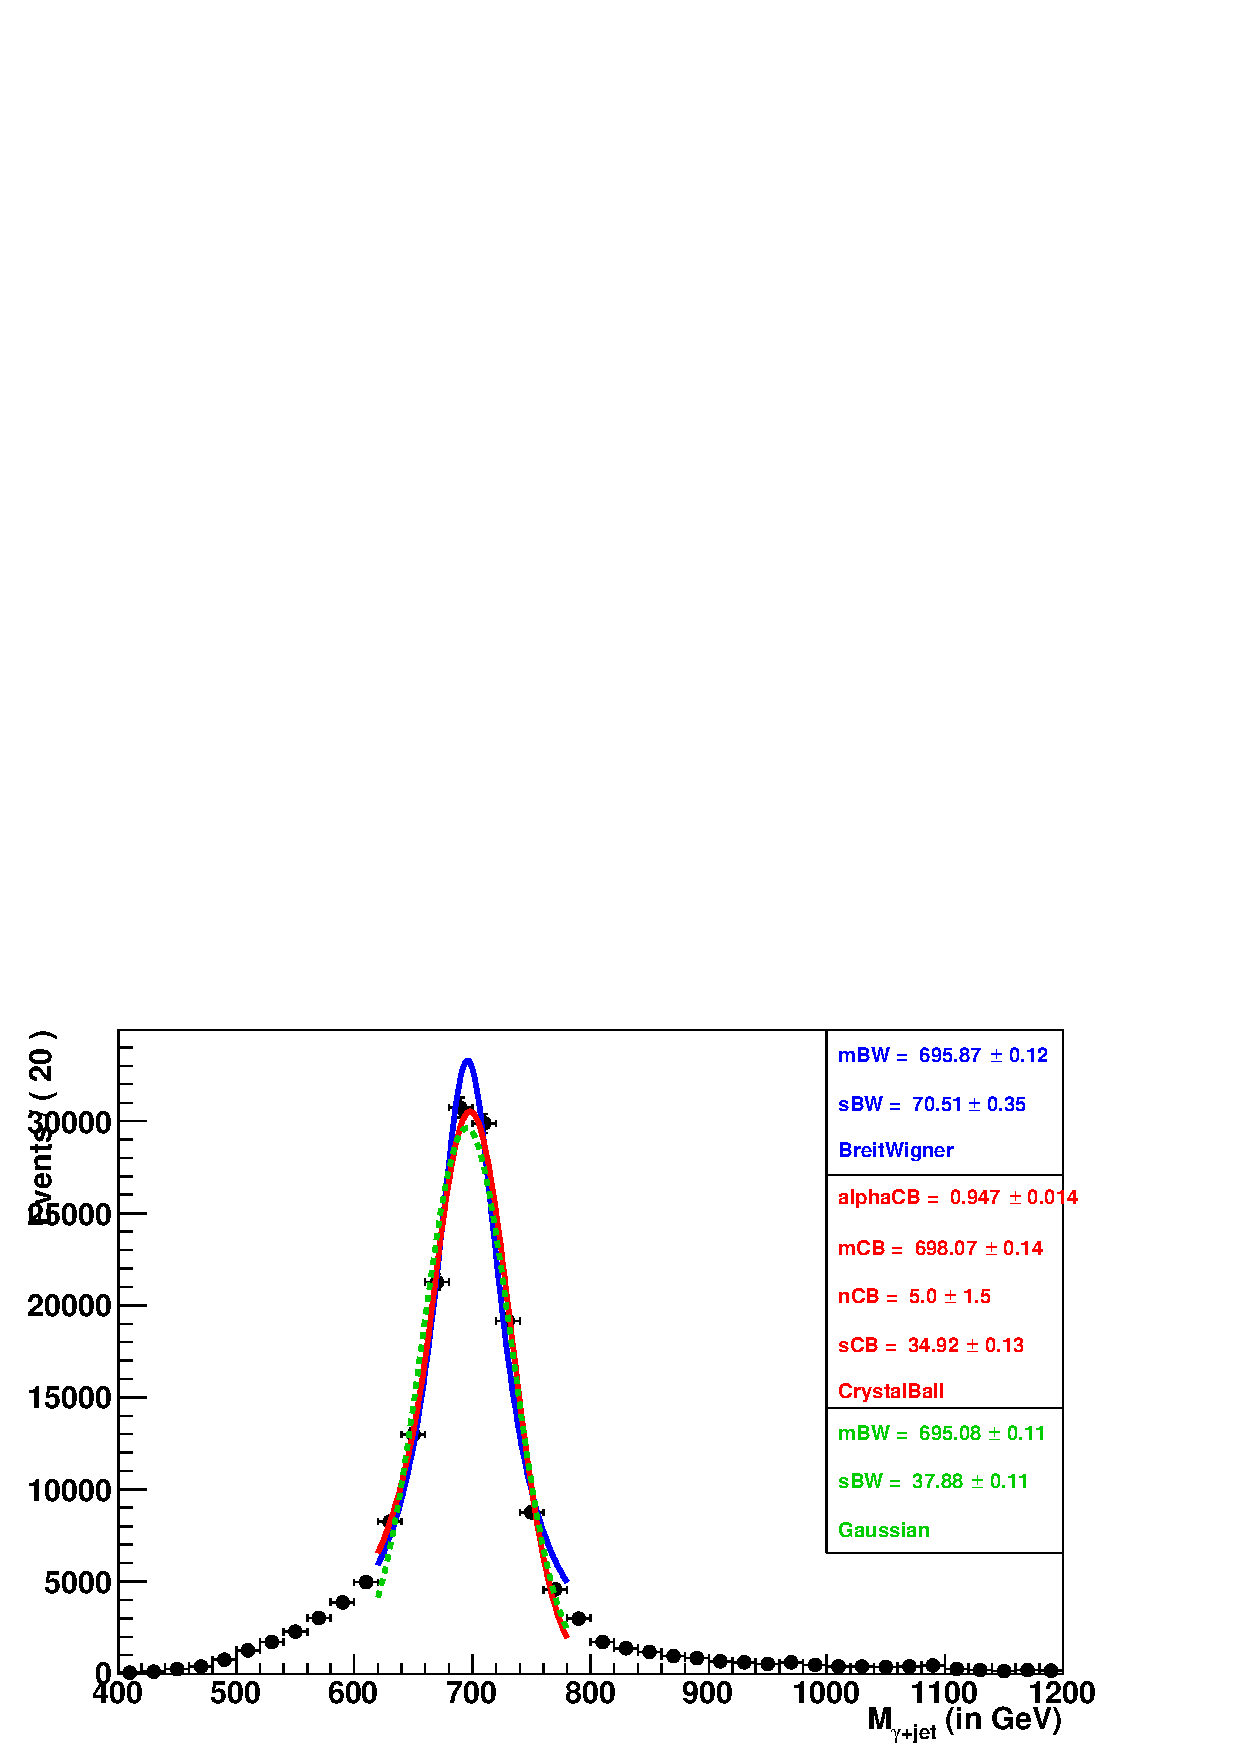
\includegraphics[width=8.0cm,height=6cm]{ch5/plots/FittingSigPlots/Qstar700_bin20.pdf}}
 \subfloat[$\mqstar=1000\unit{GeV}$]{\label{fig:FitQ1000}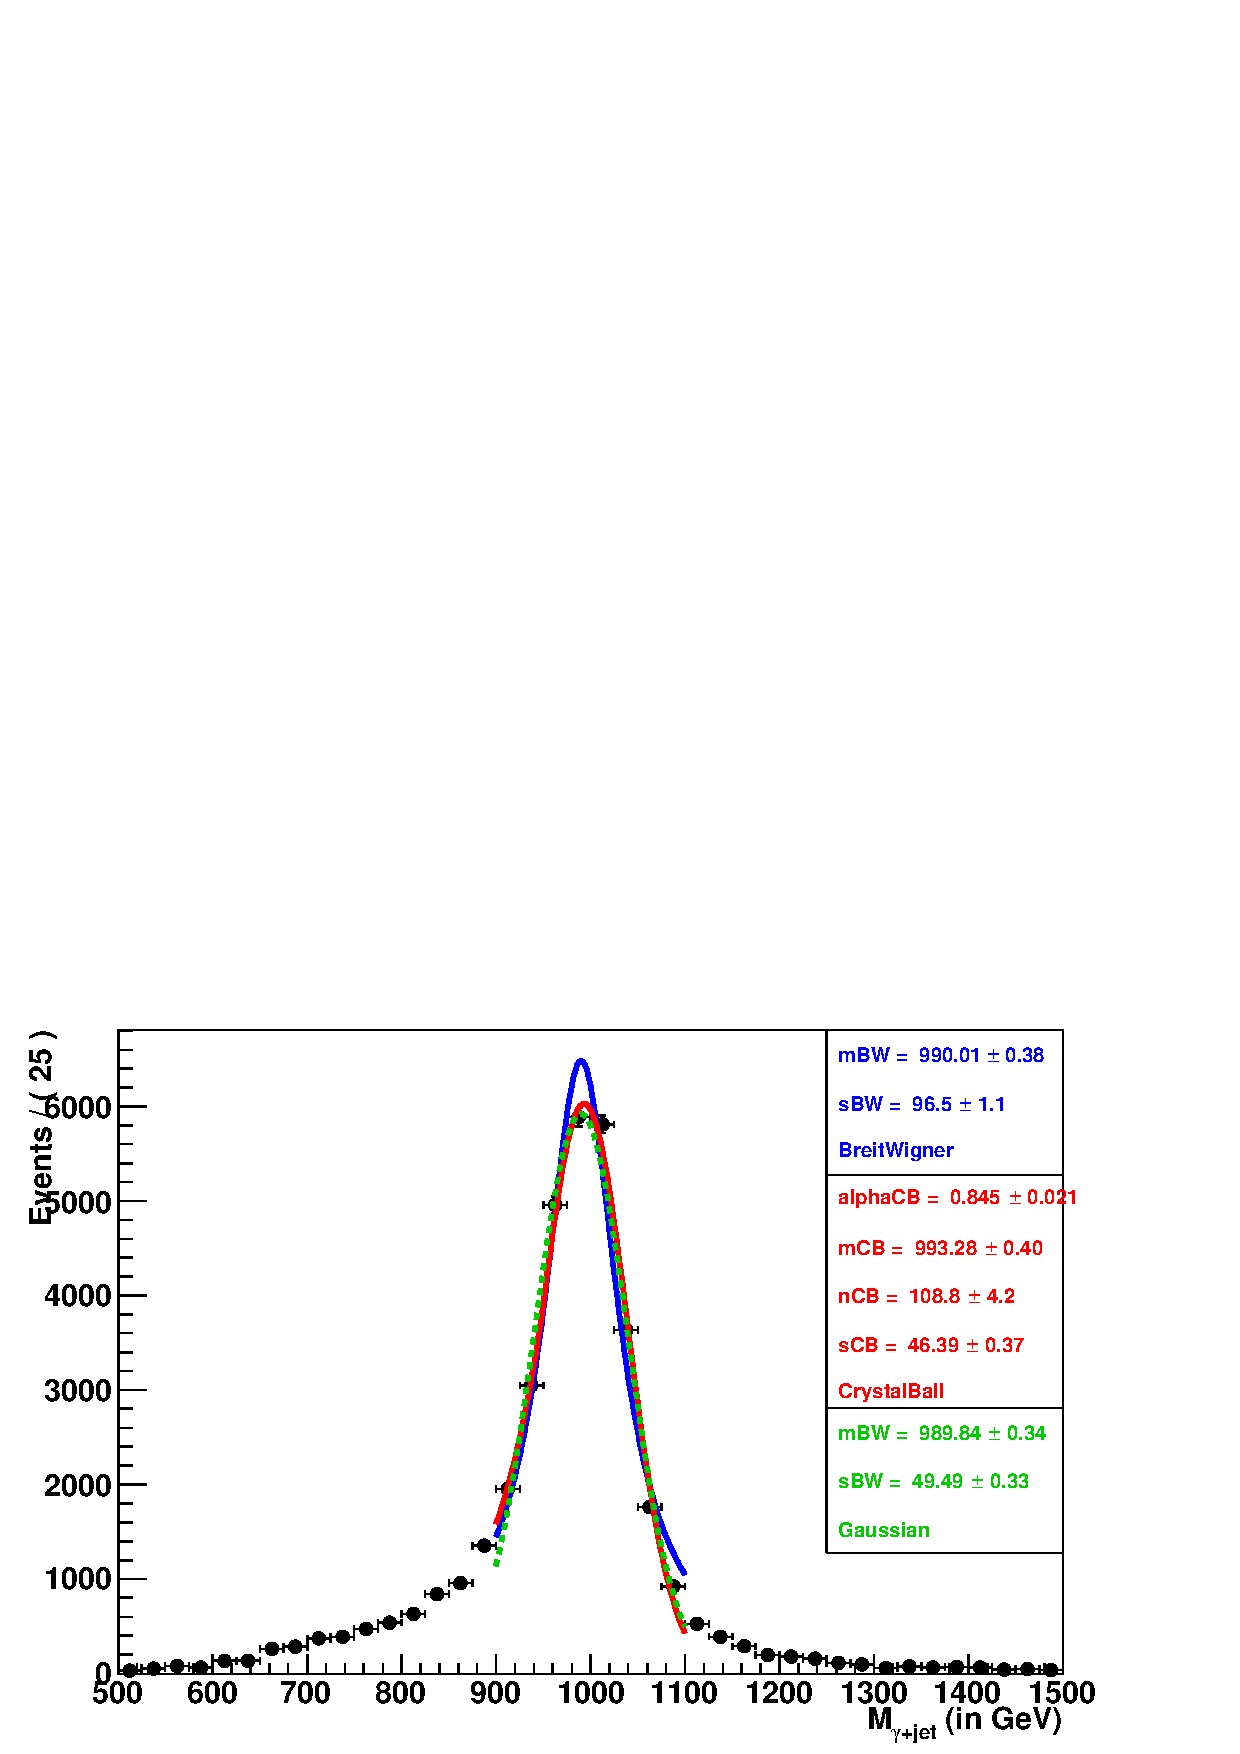
\includegraphics[width=8.0cm,height=6cm]{ch5/plots/FittingSigPlots/Qstar1000.pdf}} \\
 \subfloat[$\mqstar=1200\unit{GeV}$]{\label{fig:FitQ1200}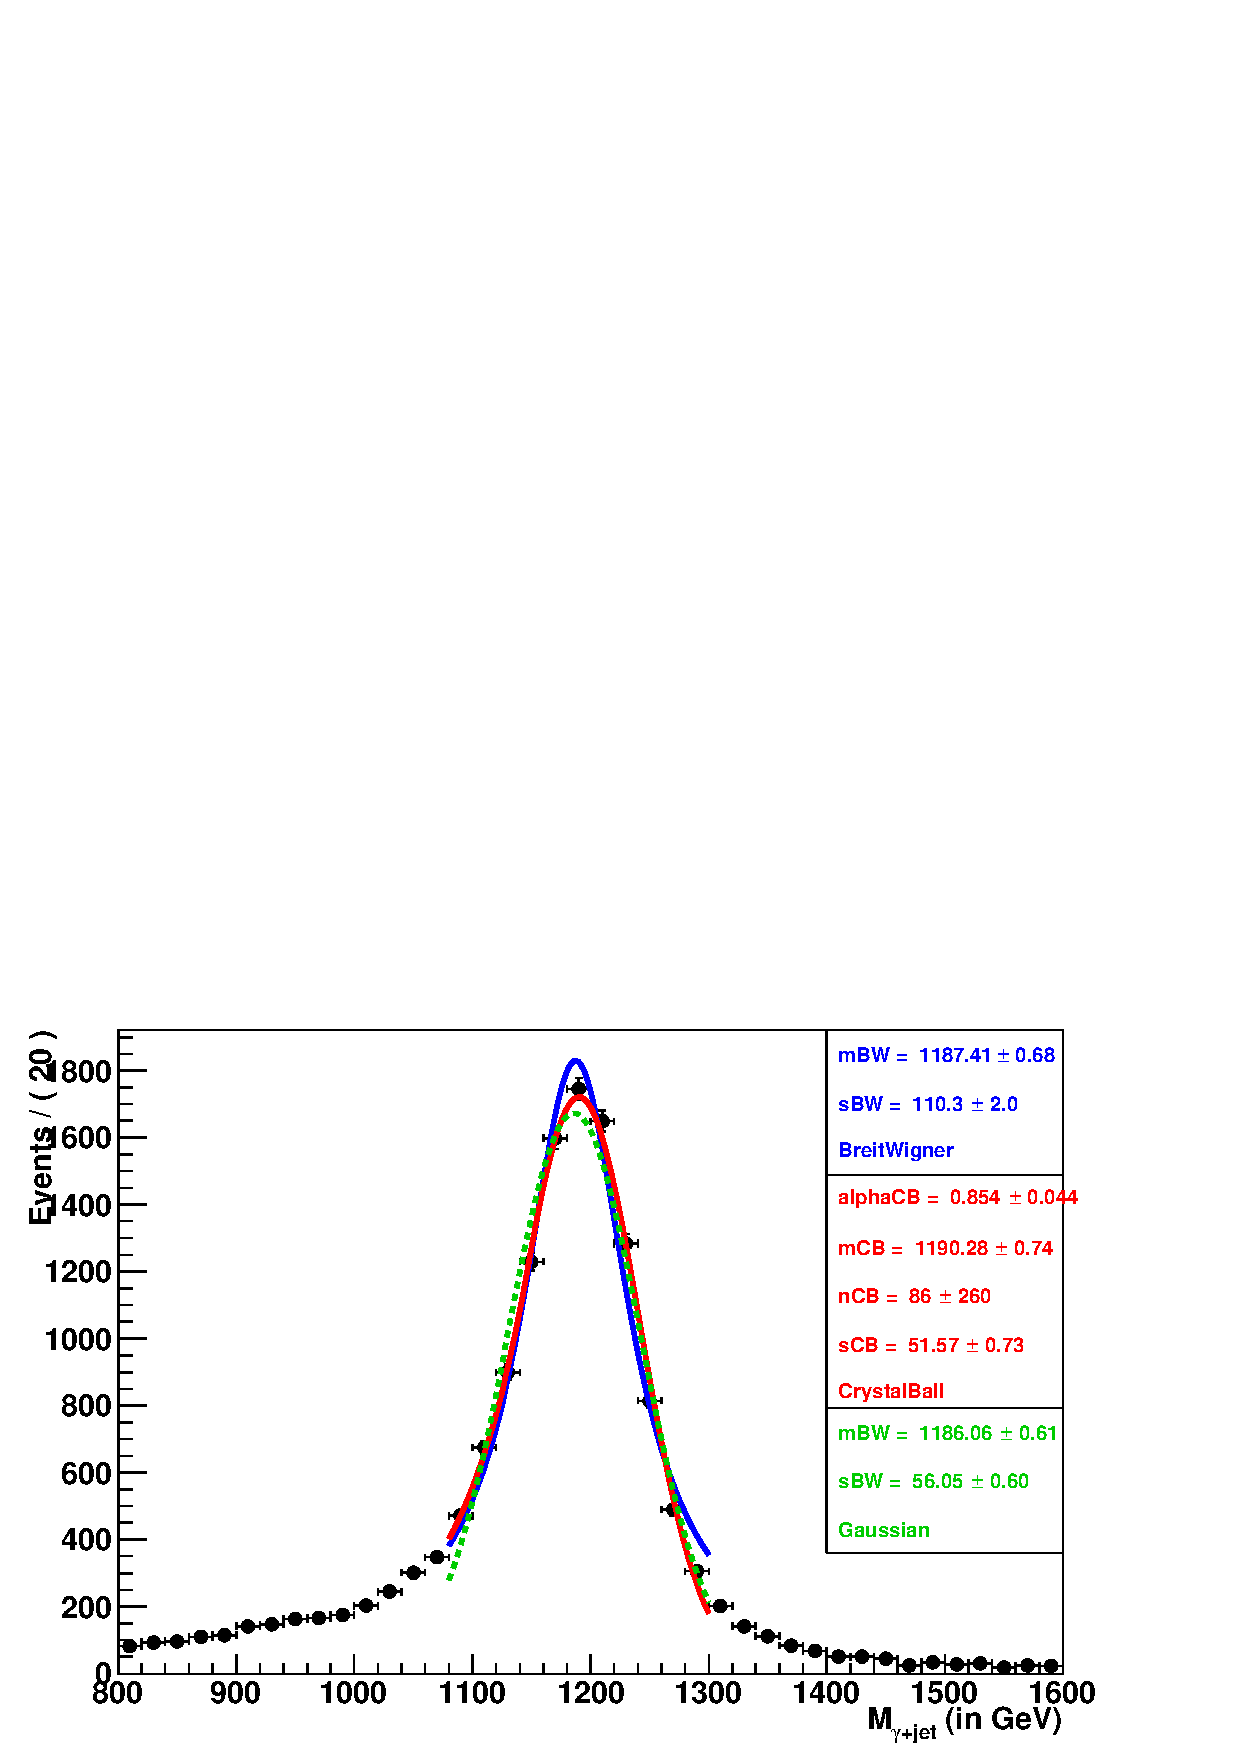
\includegraphics[width=8.0cm,height=6cm]{ch5/plots/FittingSigPlots/Qstar1200_bin20.pdf}} \\
 \subfloat[$\mqstar=1500\unit{GeV}$]{\label{fig:FitQ1500}\includegraphics[width=8.0cm,height=6cm]{ch5/plots/FittingSigPlots/Qstar1500_bin20.pdf}}
 \subfloat[$\mqstar=1700\unit{GeV}$]{\label{fig:FitQ1700}\includegraphics[width=8.0cm,height=6cm]{ch5/plots/FittingSigPlots/Qstar1700_bin25.pdf}} \\ 
 \caption{Fitting the core of \qstar invariant mass for different samples of \mqstar from 700 to 1700\unit{GeV} with $f=1.0$ using Breit-Wigner 
(Blue), Crystal-Ball (Red), and Gaussian (Green) functions to get the mass resolution of each mass point.}
 \label{fig:fitQstarMass}
\end{figure}
\begin{figure}[h!]
\centering
 \subfloat[$\mqstar=2000\unit{GeV}$]{\label{fig:FitQ2000}\includegraphics[width=8.0cm,height=6cm]{ch5/plots/FittingSigPlots/Qstar2000_bin25.pdf}} 
 \subfloat[$\mqstar=2500\unit{GeV}$]{\label{fig:FitQ2500}\includegraphics[width=8.0cm,height=6cm]{ch5/plots/FittingSigPlots/Qstar2500_bin25.pdf}} \\
 \subfloat[$\mqstar=3000\unit{GeV}$]{\label{fig:FitQ3000}\includegraphics[width=8.0cm,height=6cm]{ch5/plots/FittingSigPlots/Qstar3000_bin25.pdf}}
 \subfloat[$\mqstar=3500\unit{GeV}$]{\label{fig:FitQ3500}\includegraphics[width=8.0cm,height=6cm]{ch5/plots/FittingSigPlots/Qstar3500_bin25.pdf}} \\
 \caption{Fitting the core of \qstar invariant mass for different samples of \mqstar from  2000 to 3500\unit{GeV} with $f=1.0$ using Breit-Wigner 
(Blue), Crystal-Ball (Red), and Gaussian (Green) functions to get the mass resolution of each mass point.}
 \label{fig:fitQstarMass1}
\end{figure}
It was used to compute the mass resolution, defined as $\sigma/mean$ for various mass points of \qstar signal. The mass resolution obtained by 
fitting \qstar signal peaks with Crystal function (\eqn{\ref{eq:crystalball}}), was again fit using \eqn{\ref{eqn:massBin}} to get a functional 
form for the invariant mass binning. In \eqn{\ref{eqn:massBin}}, $M_{Res}$ refers to the actual resonance mass of the \qstar signal. 
\begin{equation}
\frac{\sigma}{Mean} = A + \frac{B}{M_{Res}}
\label{eqn:massBin}
\end{equation}
The fit to \qstar mass resolution for different mass points has been illustrated in \fig{\ref{fig:MassResolution}}. The binning obtained using this 
function, and used for different invariant mass distributions is mentioned below in an array named nMassBin[].
\begin{figure}[h!]
\centering
 \includegraphics[width=7.5cm,height=5.95cm]{ch5/plots/Fitting/Fit_SigmaMean_v1.pdf}
 \caption{Fit function to get the variable binning from resolution of signal samples.}
 \label{fig:MassResolution}
\end{figure}
{\scriptsize
\begin{verbatim}
nMassBin[102] = {1, 3, 6, 10, 16, 23, 31, 40, 50, 61, 73, 86, 100, 115, 132, 150, 169, 189, 210,
                 232, 252, 273, 295, 318, 341, 365, 390, 416, 443, 471, 500, 530, 561, 593, 626,
                 660, 695, 731, 768, 806, 846, 887, 929, 972, 1017, 1063, 1110, 1159, 1209, 1261,
                 1315, 1370, 1427, 1486, 1547, 1609, 1673, 1739, 1807, 1877, 1950, 2025, 2102, 
                 2182, 2264, 2349, 2436, 2526, 2619, 2714, 2812, 2913, 3018, 3126, 3237, 3352, 
                 3470, 3592, 3718, 3847, 3980, 4117, 4259, 4405, 4556, 4711, 4871, 5036, 5206, 
                 5381, 5562, 5748, 5940, 6138, 6342, 6552, 6769, 6993, 7223, 7461, 7706, 7959};
\end{verbatim}
}

\subsection{Choice of Fit function}\label{Se:fit}
The invariant mass distribution of both the MC simulation and data, illustrated in \fig{\ref{fig:massVarBin}} are plotted in bins of width
similar to that of the expected mass resolution of \qstar,  which varies from 4.5\% at 1\unit{TeV} to 3\% at 3\unit{TeV} as obtained in the previous
section. The MC simulation for background, while not used to compute the analysis results, is seen in \fig{\ref{fig:massVarBin}} to describe the 
data well, both in shape and yield. 

%%%-- ~\cite{Harris:2011bh}\\Review article, ~\cite{Aaltonen:2008dn}\\NLO comparison
The heart of the search for the \qstar resonance is the measurement of the \gamjet mass distribution and the estimation of the background.  
The traditional method to search for a large resonance signal used by previous experiments viz. UA2, CDF~\cite{Harris:2011bh}, is adopted,
wherein background is estimated using a smooth parameterization. One can either use the MC simulations or the parameterized fit function estimated
using the data to finally evaluate the background. In this analysis we have used the fit function to simulate the background. The advantage of using fit
function is that even though the shape and normalization may agree between the data and the MC, 
%The advantage of using a fit function over MC simulation is that, even when shape and normalization agree between the data and the simulated background, 
there are still considerable theoretical uncertainties such as PDFs, renormalization scale, etc. and experimental uncertainties such as jet energy 
scale, resolution, etc. The methodology of smooth parameterization makes use of the fact that \gamjet background always produces a smooth and monotonically decreasing 
spectrum. To extract the smoothly falling background, the \gamjet invariant mass is fit to several functional forms used in searches for resonance 
signal at previous experiments, also discussed in Ref~\cite{Harris:2011bh}. Functions that were tested to model the SM background in the best 
possible manner are:
\begin{itemize}
\item  $ F_{1}(x) = \frac{p_{0}\ast(1+x)^{p_{1}}}{x^{p_{2}+p_{3}ln(x)}} $   %% function1 
\item  $ F_{2}(x) = \frac{p_{0}\ast(1-x)^{p_{1}}}{x^{p_{2}+p_{3}ln(x)}} $   %% function2
\item  $ F_{3}(x) = \frac{p_{0}}{{p_{1}+p_{2}x+x^{2}}^{p_{3}}} $  %% function3
\item  $ F_{4}(x) = \frac{p_{0}(1-x+p_{3}x^{2})^{p_{1}}}{m^{p_{2}}}   $  %% function4
\item  $ F_{5}(x) = \frac{p_{0}}{(x+p_{1})^{p_{2}}} $  %% function5
\end{itemize}
where $x=m/\sqrt{s}$, $m$ being the \gamjet invariant mass, $\sqrt{s}$ is the center-of-mass energy, and $p_0$, $p_1$, $p_2$, and $p_3$ are the fit 
parameters. These parameterizations are motivated by LO QCD. The term $x^{p_{2}}$ or $m^{p_{2}}$ in the denominator mimics the  QCD matrix element 
mass dependence and was introduced in searches at UA2 experiments~\cite{Harris:2011bh}. The term $(1\pm{x})^{p_{1}}$ in the numerator mimics the
\begin{figure}[h!]
\centering
\subfloat[Fit to data with different fit functions described in the text.]{\label{fig:FitDiffFunction}
      \includegraphics[width=13cm,height=8cm]{ch5/plots/Fitting/FitToData_DifferentFunctions.pdf}}  \\
\subfloat[Residuals for all the fit function on the same scale.]{\label{fig:FitDifFunctionResiduals}
      \includegraphics[width=13cm,height=8cm]{ch5/plots/Fitting/Residuals_FitToData_DifferentFunctions.pdf}}
\caption{Fit \gamjet invariant mass in data using different fit function.}
\label{fig:DiffFitFunc}
\end{figure}
mass dependence of the parton distributions at an average fractional momentum of $m/\sqrt{s}$ and was introduced by CDF~\cite{Harris:2011bh}. 
The $p_{3}$ term was added in order to model the data at high invariant mass.

Fit to data with the above set of functions is shown in \fig{\ref{fig:FitDiffFunction}}, while their residuals, \ie, (Data - Fit)/$\sigma_{Data}$
are reported in \fig{\ref{fig:FitDifFunctionResiduals}}. Though, almost all the functions describe the data well, the function $F_{2}$, which
has a good comparison with a full NLO QCD calculation from fastNLO was chosen for this study as shown in Ref~\cite{Aaltonen:2008dn}. This function
is also used by the ATLAS experiment for resonance search in the \gamjet and the dijet final states~\cite{ATLAS:2011ai,Aad:2013cva} and the CMS 
experiment in the dijet final state~\cite{Chatrchyan:2013qha}. It also had a slightly better $\chi^{2}/ndf$ and less fluctuations in all the mass bins 
when compared with other four functions as can be seen in \fig{\ref{fig:FitDiffFunction}}, where $\chi^{2}/ndf$ for all the fit functions are listed
in the top right corner of the plot. 

%The analysis juxtapose the observed data with the background obtained from an analytic fit to the data plus the possible presence of a \qstar signal. 
The modeling of the \gamjet background is based on the smooth parametrization $F_{2}$,
\begin{equation}
\frac{d\sigma}{dm} = \frac{P_{0}(1-m/\sqrt{s})^{P_{1}}}{(m/\sqrt{s})^{P_{2}+P_{3}ln(m/\sqrt{s})}}
\label{Eq:fitFunc}
\end{equation}
%%p0=2.74277e-03, p1=3.33455e+00, p2=8.06973e+00, p3=7.47310e-01
where \sqrteighttev, and $P_0=2.74277\times10^{-3}\pm1.199\times10^{-4}$, $P_1=3.33455\pm1.831\times10^{-1}$, $P_2=8.06973\pm1.745\times10^{-2}$,
 and $P_3=7.47310\times10^{-1}\pm5.88315\times10^{-3}$ are the 4-parameters used to describe the background. The fit probability tells us whether the data is smooth, or not, which is the first test for the presence of a resonance. To check the stability of this function for fit to data, and avoid any 
bias from statistically rich low mass region, different mass range were chosen, and were fit using the same function. The result of the fit with 
different mass 
ranges is shown in \fig{\ref{fig:DiffRangeFit}}.

\begin{figure}[h!]
\centering
 \subfloat[Fit to data for $F_2$ over different mass range]{\label{fig:FitDiffRange}
      \includegraphics[width=13cm,height=8cm]{ch5/plots/Fitting/FitToData_DifferentRange.pdf}} \\
 \subfloat[Residuals for fit to data for $F_2$ over different mass range]{\label{fig:FitDifRangeResiduals}
      \includegraphics[width=13cm,height=8cm]{ch5/plots/Fitting/Residuals_FitToData_DifferentRange.pdf}}
 \caption{Fit to data with different fit ranges.}
\label{fig:DiffRangeFit}
\end{figure}
The difference between the data and the fit, referred to as residuals, is used to estimate the significance of the largest upward fluctuation in 
the data interpreted as a narrow resonance. The parametrization in \eqn{\ref{Eq:fitFunc}}, gives a good description of both the observed data and
simulated background, as shown in \fig{\ref{fig:massFit}}. The resulting fit has a $\chi^{2}$ of 20.57 for 34 degrees of freedom. The residual 
difference between the fit and observed data for each mass bin, as shown at the bottom of \fig{\ref{fig:massFit}}, do not show significant difference
between the two. The largest fluctuations in the data are seen  at $\sim1.5$ and 2.3\unit{TeV} of mass but are not significant enough to claim any
evidence of a resonance and are consistent with background fluctuation. \Fig{\ref{fig:massFit}} also shows simulated \qstar resonance peaks for 1.0
and 1.5\unit{TeV} with $f=1.0$ and a resonance peak at 2.5\unit{TeV} with $f = 0.5$.
\begin{figure}[h!]
\centering
 \includegraphics[width=15cm,height=11.5cm]{ch5/plots/DataMC/InvMass_DataFitMC_Paper_TeV.pdf}
 \caption{The \gamjet invariant mass spectrum from data, the result of the fit with fit error, and residuals.}
\label{fig:massFit}
\end{figure}

The event with highest \gamjet invariant mass in data was observed at 2934\unit{GeV}. The event display for the event with highest mass
after passing the full selection criteria was made using cmsShow package~\cite{Web:cmsShow} in several planes viz. $r-\phi$, $\rho-z$, and 
3-dimensional, and is reported in \fig{\ref{fig:EventDisplay}}. It is a very well balanced \gamjet event from: Run Number-208551, 
Lumisection-474, and Event Number-755901799. The \pt of the photon reconstructed in this event was found to be 1361\unit{GeV} and that of jet was 
1280\unit{GeV}. The event was recorded by the CMS detector on 5$^{\mathrm{th}}$ December 2012 and thus could be found in Run2012D dataset. 
\begin{figure}[h!]
\centering
 \subfloat[$r-\phi$ plane]{\includegraphics[width=11cm,height=7.7cm]{ch5/plots/EventDisplay/R_Phi.pdf}} \\
% \subfloat[$\rho-z$ plane]{\includegraphics[width=8.2cm,height=8cm]{ch5/plots/EventDisplay/Rho_Z.pdf}}
 \subfloat[$\rho-z$ plane]{\includegraphics[width=8cm,height=5.7cm]{ch5/plots/EventDisplay/Rho_Z.pdf}} \\
% \subfloat[3-dimensional view]{\includegraphics[width=8.2cm,height=8cm]{ch5/plots/EventDisplay/3D_GifView.pdf}}
 \subfloat[3-dimensional view]{\includegraphics[width=8cm,height=5.7cm]{ch5/plots/EventDisplay/3D_GifView.pdf}} 
 \caption{Graphic display for highest \gamjet invariant mass event in different geometric planes, with \mgamjet = 2934.4\unit{GeV}, $p^{\gamma}_{T}$ = 1361.3\unit{GeV} and $p^{jet}_{T}$ = 1280.2\unit{GeV}.}
\label{fig:EventDisplay}
\end{figure}

\section{Interpolation technique}\label{Se:InterpolationTech}
When searching for new resonances or particles, \emph{a priori}, we do not have the knowledge of mass point where to expect a peak, and hence need 
to scan the entire mass range possible. For this study only 20 \qstar signal mass points were generated using event generators ranging from 700\unit{GeV} to 4.5\unit{TeV}, 11 for coupling $f = 1.0$ and 9 for $f=0.5$. 
\begin{figure}[h!]
\centering
 \subfloat[]{\label{fig:XDistGen}\includegraphics[width=8cm,height=5.6cm]{ch5/plots/InterpolationPlots/XDistribution.pdf}}
 \subfloat[]{\label{fig:XDistInt}\includegraphics[width=8cm,height=5.6cm]{ch5/plots/InterpolationPlots/XDistributionWithInterpolated.pdf}}
 \caption{$X$ distribution for excited quark with different mass points for generated and Interpolated samples.}
 \label{fig:XDist}
\end{figure}
To study the intermediate mass region, the shape of resonances at mass values that were not generated are obtained using an interpolation 
technique~\cite{Interpolation}, wherein information is extracted from the nearest neighboring generated mass points. Here, at first a new 
parameter, $X = \frac{\mgamjet}{M_{Res}}$ is defined, where, \mgamjet  is the \gamjet mass and $M_{Res}$ is resonance mass. The $X$ distribution 
is computed for all the generated \qstar mass points and the comparison of these distributions for various \qstar mass points is reported in 
\fig{\ref{fig:XDistGen}}. Then, $X$ distributions for the mass points that has to be interpolated were generated using \eqn{\ref{eq:interpolation}}. 
If a resonance mass $M$ lies between the generated mass point $M_{A}$ and $M_{B}$, (A $<$ B) following equation is applied to obtain the $X$ distribution,
\begin{equation}\label{eq:interpolation}
Prob_{M}(X) = Prob_{A}(X) + [ Prob_{B}(X) - Prob_{A}(X) ] \cdot \frac{M - M_{A}}{M_{B} - M_{A}}
\end{equation}
where, $Prob_M(X)$, gives the probability of a mass point defined by $X$. For example, to generate distribution of a resonance with mass of
1.7\unit{TeV}, the first thing is to search for its nearest generated masses. Since 1.5\unit{TeV} and 2.0\unit{TeV} are the immediate neighbors, they 
form $M_{A}$ and $M_{B}$, leaving the above equation to the following,
\begin{equation}
Prob_{1.7\unit{TeV}}(X) = Prob_{1.5TeV}(X) + [ Prob_{2.0TeV}(X) - Prob_{1.5}(X) ] \cdot \frac{1.7 - 1.5}{2.0 - 1.5} 
\end{equation}
The comparison of $X$ distribution of the interpolated mass points with those that were generated is shown in \fig{\ref{fig:XDistInt}}. Lastly, 
the $X$ distribution for the interpolated mass point was multiplied with the respective resonance mass value and converted to variable \gamjet 
binning using \eqn{\ref{eqn:massBin}} to obtain the final \qstar resonance mass shape at respective mass value. The fully interpolated mass 
point for some of the mass values is shown in \fig{\ref{fig:ComGenIP}}, where, solid lines are for the generated samples and dotted lines represent
interpolated mass shapes. 
\begin{figure}[h!]
\centering
 \includegraphics[width=15cm,height=8cm]{ch5/plots/InterpolationPlots/InterpolatedSample.pdf}
 \caption{Comparison of \qstar resonance shapes for the generated and interpolated samples. The solid lines are from the generated samples (q*) while 
dotted lines represent interpolated samples (I.M).}
 \label{fig:ComGenIP}
\end{figure}
\begin{figure}[h!]
\centering
% \includegraphics[width=15cm,height=8cm]{ch5/plots/InterpolationPlots/GenVsIP_massPlot_2500GeV.pdf}
 \includegraphics[width=15cm,height=8cm]{ch5/plots/InterpolationPlots/GenVsIP_massPlot_1TeV_2p5TeV.pdf}
 \caption{Comparison of \qstar resonance shape for generated (solid lines) and interpolated (dotted lines) excited quark at 1.0 and 2.5 TeV.}
 \label{fig:ComGenIP2500}
\end{figure}

To verify this technique a closure test was performed in which an already generated mass point, viz. 2.5\unit{TeV}, was chosen to be interpolated 
using its immediate neighbors, viz. 2.0 and 3.0\unit{TeV}. The shape of the interpolated 2.5\unit{TeV} mass point was then compared with its
generated shape and a good agreement was observed, as reported in \fig{\ref{fig:ComGenIP2500}}. A similar comparison for \qstar with mass 
1.0\unit{TeV} is also shown in the same figure, which is interpolated using 0.7 and 1.2\unit{TeV} generated \qstar sample. To add weight to this 
test, observed cross section was also evaluated using both the shapes, result of which are described in \sectn{\ref{Se:optimization}}.


\section{Systematic Uncertainties}\label{Se:SysUnc}
There are various sources of systematic uncertainties in this analysis, such as those due to reconstructed objects identification 
inefficiencies, energy scales, measurement in luminosity, etc. In this section, I describe the most significant of them and they 
are listed below:
\begin{itemize}
\item Photon and Jet Energy Calibration Scale
\item Photon and Jet Energy Resolution 
\item Final State Radiations 
\item Background Shape
\item Theoretical Uncertainty
\item Pile-up Uncertainty
\item Luminosity
\end{itemize}

Only Background shape uncertainty is included in background since the background shape is derived from data and the rest of the uncertainties are 
considered for the resonance signal shapes alone.

\subsection{Photon and Jet Energy Calibration Scale}
The energy measured in calorimeters is different from the true particle-level energy. The difference is caused primarily by the non-uniform and 
non-linear response of the calorimeters. %If the simulation produces photons or jets with very high response, the true position of the expected 
%peak of a given \gamjet resonance mass would appear at lower mass than predicted by simulation in the actual measured \gamjet mass spectrum. 
Therefore, corrections are made to the energy scale of the reconstructed photons and jets. 
\begin{figure}[h!]
\centering
 \includegraphics[width=10cm,height=7cm]{ch5/plots/Systematics/JES_Sys.pdf}
 \caption{Uncertainty in jet Energy Scale as a function of mass.}
 \label{fig:JESsys}
\end{figure}
\begin{figure}[h!]
\centering
 \includegraphics[width=10cm,height=7cm]{ch5/plots/Systematics/PES_Sys.pdf}
 \caption{Uncertainty in photon energy scale as a function of mass.}
 \label{fig:PESsys}
\end{figure}

%The photon energy scale (PES)~\cite{Chatrchyan:2011ds,Chatrchyan:2013fya} and jet energy scale (JES)~\cite{Chatrchyan:2011ds} uncertainties were
%considered only for the simulation of the \qstar resonance, as the background component comes directly from the signal+background fit to data and
%therefore, have the same scales as the data. 
The photon energy scale (\gls{PES}) uncertainty~\cite{Chatrchyan:2011ds,Chatrchyan:2013fya} was found to be about 1.5\%, while the jet energy scale (\gls{JES}) 
uncertainty~\cite{Chatrchyan:2011ds} was found to vary between $1.0-1.4\%$. The effect of the photon and jet energy scale uncertainty was studied on 
the \gamjet mass spectrum of the \qstar signal, wherein the four-momenta of photon and jet is varied by $1\pm\text{uncertainties}$ and is reported in 
\fig{\ref{fig:JESsys}} and \ref{fig:PESsys}. It was found to have an effect of 0.75\% on the \qstar resonance shape in the case of photons and 
0.8\% for jets. 

\subsection{Photon and Jet Energy Resolution}
If the \gamjet mass resolution of the simulated \qstar signal is wider or smaller than what we expect, it may be harder to find a resonance, as it 
may either spread over a large number of bins or get contained in just a few of them. So, it is important to incorporate the uncertainty due to 
energy resolution. The uncertainty on the jet energy resolution(JER)~\cite{Chatrchyan:2011ds} and photon energy resolution(PER)~\cite
{Chatrchyan:2013dga} was taken to be 10\% and 0.5\%, respectively. The uncertainty in \gls{JER} and \gls{PER} translates into a relative uncertainty of 5\% on the 
\gamjet mass and is propagated to the search by changing the width of the resonance shape, which results in slight stretching or shrinking of the 
resonance shape itself.

\subsection{Final State Radiations}
The initial state radiation (\gls{ISR}) and the final state radiation (\gls{FSR})  could also affect the shape of \qstar resonances. The effect of ISR is 
small and mostly contained in the low mass tail but FSR could affect the determination of the mean and width of these resonances significantly. 
The effect of FSR depends on the choice of the scale. Within \pythia~\cite{Sjostrand:2006za}, this is controlled by a parameter, PARJ(81), 
set at 0.29 for the nominal scenario. To estimate the uncertainty due to FSR, the parameter value was scaled by a factor of 2.0 and 0.5. The change 
in mean was found to be $\pm$0.5\% as reported in 
%---------------TABLE FOR MC samples-------------------
\begin{table}[h!]
  \begin{center}
 \resizebox{\columnwidth}{!}{
   \begin{tabular}{|l|c|c|c|c|c|}
     \hline
     {\bf FastSim Signal} & {\bf PARJ(81)}  & {\bf Mean (GeV) } & {\bf Width (GeV)} & {\bf Expected Limit} & {\bf Observed Limit}  \\
     \hline
     \hline
     1 TeV Down     & 0.145    & 988.48      & 57.08       & 0.0154572      & 0.00885582 \\
     1 TeV Nominal  & 0.29     & 993.08      & 61.35       & 0.0153808      & 0.00980415 \\
     1 TeV Up       & 0.58     & 995.6       & 59.15       & 0.0161674      & 0.00927311 \\  
     \hline
     \hline
     3 TeV Down     & 0.145    & 2941.81     & 149.68      & 0.000457463    & 0.00034185 \\
     3 TeV Nominal  & 0.29     & 2951.8      & 144.25      & 0.000457362    & 0.000352528 \\
     3 TeV Up       & 0.58     & 2958.39     & 144.70      & 0.000473748    & 0.000365025 \\
     \hline
   \end{tabular}
}
  \caption{Effect of change in Final state radiations on the mean and width of FASTSIM q* shapes at 1 TeV and 3 TeV.}
  \label{Table:FSRUnc}
 \end{center}
\end{table}

\tab{\ref{Table:FSRUnc}}, for both a low and a high mass signal. The change in width was found to be 7\% (4\%) for 1\unit{TeV} (3\unit{TeV}) \qstar 
mass shapes generated using FASTSIM~\cite{Giammanco:2014bza}. In \tab{\ref{Table:FSRUnc}}, `Down' refers to scaling by factor 0.5 while, `Up' means by 
a factor of 2.0.

\subsection{Background Shape Uncertainty}
To estimate the uncertainty due to the background fit, different functional forms were tested to parametrize the data, as shown in 
\fig{\ref{fig:DiffFitFunc}}. The statistical uncertainty in the prediction of fit using the chosen function was estimated to be 1\% at 1\unit{TeV}
and about 30\% at 3\unit{TeV}. A signal-plus-background fit to  the data was performed to identify a reasonable starting point for each of the four 
parameter values. Covariance matrix of the 4 background parameters ($P_0$, $P_1$, $P_2$, $P_3$) was diagonalized and the variations of the original 
4 parameters along the 4 eigenvectors of the covariance matrix were introduced as nuisance parameters. These nuisance parameters were integrated
over a $\pm7\sigma$ range, around the best fit values, where $\sigma$ is the square root of the corresponding eigenvalue of the covariance matrix. 
It had been verified that the result remains stable if a bigger integration interval was chosen.

\subsection{Theoretical Uncertainty}
%The uncertainty due to the choice of parton density functions has been estimated using method described in \cite{Web:PDFUnc} as per the PDF4LHC 
%recommendations~\cite{Botje:2011sn,Alekhin:2011sk,Ball:2012cx}. The PDF Uncertainty were evaluated for \qstar signal simulation only and not for the 
%background as it was extracted using a data driven technique. Uncertainty for different signal mass points is summarized in \tab{\ref{Table:pdfUnc}}. 
Theoretical uncertainties, here, refer to the choice of factorization and renormalization scales. These were varied by a factor of 0.5 and 2.0, separately, to estimate the variation in the signal cross section for different resonances masses. The uncertainties in the signal due to the 
variation in scales were found to be about 4\%.
%\begin{table}[h]
\centering
 \begin{tabular}{|c|c|c|c||}
  \hline
    \mqstar (in TeV)  & MSTW2008nlo68cl  & NNPDF20  & cteq66 \\
    \hline
    0.7  & 2.73 $\pm$ 0.23 & 2.847 $\pm$ 0.27 & 1.71 $\pm$ 0.22 \\
    1.0  & 2.31 $\pm$ 0.24 & 2.508 $\pm$ 0.27 & 1.69 $\pm$ 0.24 \\
    1.2  & 1.97 $\pm$ 0.25 & 2.544 $\pm$ 0.27 & 1.48 $\pm$ 0.25 \\
    1.5  & 2.22 $\pm$ 0.25 & 2.238 $\pm$ 0.26 & 1.08 $\pm$ 0.28 \\
    1.7  & 2.12 $\pm$ 0.26 & 1.962 $\pm$ 0.26 & 1.83 $\pm$ 0.31 \\
    2.0  & 2.03 $\pm$ 0.19 & 2.048 $\pm$ 0.18 & 1.73 $\pm$ 0.24 \\
    3.0  & 2.09 $\pm$ 0.19 & 2.071 $\pm$ 0.14 & 1.51 $\pm$ 0.35 \\
    3.5  & 1.94 $\pm$ 0.24 & 1.852 $\pm$ 0.27 & 1.42 $\pm$ 0.23 \\
    \hline
    \hline
   \end{tabular}
   \caption{PDF Uncertainity for signal samples with respect to three different PDFs.}
   \label{Table:pdfUnc}
\end{table}



\subsection{Pileup Uncertainty }
A central value for the total inelastic cross section of 69.4\unit{mb}\cite{Web:Pileup,CMS-PAS-LUM-13-001} has been used for \pp collisions at 
8\unit{TeV}. The number of interactions in the data is estimated from the measured luminosity in each bunch crossing times the total inelastic cross 
section. A variation of $\pm$5\%  in the number of interactions has been done to cover the uncertainties due to the pileup reweighting. This
includes an additional $\sim3\%$ uncertainty to cover all the physics aspects of the pileup simulation. The effect of pileup uncertainty on the 
product (acceptance $\times$ efficiency) of \qstar signal samples were found to be $\sim$0.3\%.

\subsection{Luminosity}
The total uncertainty on the integrated luminosity\cite{CMS-PAS-LUM-13-001} delivered to the CMS experiment by the LHC in \pp collisions
for the 2012 physics run was estimated to be 2.6\%.

\section{ Limit setting procedure }
As no significant excess is observed in data with respect to the background expectations, we proceed to set upper limits on the cross section 
of excited quarks in the \gamjet channel. A Bayesian technique~\cite{Beringer:1900zz} based on a binned likelihood method is used to search for 
the \qstar resonances. The binned likelihood uses three distributions in the \gamjet invariant mass: data, background, and signal. For each 
\gamjet invariant mass bin, $i$,
\begin{itemize}
\item Signal: number of events from \qstar signal simulated samples, $N_i(S)$.
\item Data: measured number of events in data, $n_i$.
\item Background: expected number of events from the background fit, $N_i(B)$.
\end{itemize}

The normalization of the \qstar signal is multiplyied with a normalization parameter $\alpha$, and added in background to obtain
the mean number of expected events $\mu_i$ , for each \gamjet invariant mass bin $i$ :
%The normalization of the signal at this point was arbitrary. It could be a normalized distribution or a distribution in number of events. 
%The size of \qstar signal was multiply by the parameter, $\alpha$ to get the mean number of expected events, $\mu_i$ , for each 
%\gamjet invariant mass bin $i$ :
\begin{equation}
\mu_{i} = \alpha N_{i}(S) + N_{i}(B)
\end{equation}
The likelihood, $\mathcal{L}(n|\mu)$, of observing $n_i$ events when $\mu_i$ are predicted is given by Poisson statistics :
\begin{equation}
\mathcal{L}(n|\mu) = \prod_{i=1}^{\text{Total Bins}}\frac{\mu^{n_{i}}_{i}e^{-\mu_{i}}}{n_{i}!}
\end{equation}

The limit code~\cite{Web:Limit} is based on the ROOT TMinuit class. The bin width size is approximately of the \gamjet mass resolution, and gradually
increases as a function of mass according to the \gamjet mass resolution. The binned likelihood $\mathcal{L}$ is used to evaluate the number 
of expected background events in each bin by integrating the chosen fit function over the bin width. The resulting fit function with the signal 
cross section set to zero is used as the background hypothesis. This provides the expected number of background events in the $i$th \gamjet mass bin, 
$N_{i}(B)$. The number of signal events in the same mass bin, $N_{i}(S)$, comes from the signal histogram templates. For the mass points for which 
\qstar signal samples were not simulated using event generators, signal templates were taken using the interpolated samples as described 
in~\sectn{\ref{Se:InterpolationTech}}. We assume a flat prior in normalization parameter $\alpha$, which is the same as a flat prior in the 
resonance cross section. The likelihood function is multiplied by the flat prior in cross section, $P(\sigma)$, and normalized to give a posterior 
probability density in cross section:
\begin{equation}
P_{post}(\sigma) = \frac{\mathcal{L}(n|\mu)P(\sigma)}{\int_{0}^{\infty}\mathcal{L}(n|\mu)P(\sigma)d\sigma}
\end{equation}

Log-normal prior distribution functions were used~\cite{Web:stat} to model the systematic uncertainties which are treated as nuisance parameter. 
The posterior probability density was calculated as a function of signal cross section for resonances with masses starting from 0.7\unit{TeV} 
to 4.5\unit{TeV} in steps of 100\unit{GeV}. Finally, the 95\% confidence level upper limit on the cross section, $\sigma_{95}$ were calculated 
from the posterior probability density as follows:
\begin{equation}
\int_{0}^{\sigma_{95}}P_{POST}(\sigma)d\sigma = 0.95
\end{equation}

The systematic uncertainties in JES, PES, JER, PER, FSR, in the integrated luminosity, and in the correction factors are used in the limit 
setting procedure as nuisance parameters and affect only the signal. They were used to evaluate model independent limits on $\sigma\times\mathcal{B}$.
%To test the limit setting procedure a signal injection test was performed which is reported in the following \sectn{\ref{Se:SigInjTest}}.
%
%\subsection{Signal Injection test}\label{Se:SigInjTest}
%To verify the limit setting procedure, a signal injection test was performed. A Gaussian signal was generated with input cross-section
%$\sim0.004\unit{pb}$ having widths and expected number of events similar to that of \qstar with mass 2.5\unit{TeV}. The background was taken 
%from the fit to data as done in the analysis. The background-plus-signal shape was fluctuated using Poisson statistics to generate the 
%\begin{figure}[h!]
%\centering
% \subfloat[Pseudo-data]{\label{fig:PseudoData}\includegraphics[width=8cm,height=5cm]{ch5/plots/SignalInjectionTest/2500TeV_SIT.pdf}} \\
%%%% \subfloat[Zoomed pseudo-data]{\label{fig:ZoomedPseudoData}\includegraphics[width=8cm,height=5cm]{ch5/plots/SignalInjectionTest/2500TeV_SIT_ZOOM.pdf}} \\
% \subfloat[Observed upper limit]{\label{fig:ObservedUpperLimit}\includegraphics[width=8cm,height=5cm]{ch5/plots/SignalInjectionTest/IncSyst_ObsExpect_SIT_25TeV.pdf}}
% \subfloat[Observed limit for all pseudo data]{\label{fig:ObservedLimitAllPD}\includegraphics[width=8cm,height=5cm]{ch5/plots/SignalInjectionTest/SpB_vs_B.pdf}}
% \caption{Signal Injection test}
%%%%%\label{fig: Signal Injection test}
%\end{figure}
%pseudo-data. About 200 set of Poisson fluctuated pseudo-data were generated, with one such pseudo data is shown in \fig{\ref{fig:PseudoData}}. 
%\Fig{\ref{fig:ObservedUpperLimit}} shows the expected and observed limits from the generated pseudo data, which results in a bump in the
%observed cross section upper limits ($>5\sigma$) at 2.5\unit{TeV}. The shape of the excess in observed limit is quite broad and consistent with the 
%signal shape as expected in \qstar signal at 2.5\unit{TeV}. Some local excess at $\sim1.6\unit{TeV}$ for this particular pseudo-data was also seen
%due to upward fluctuation in the pseudo-data at this value. For randomly generated 200 such pseudo-data, observed limit with 95\% CL upper limit for
% signal-plus-background (RED) and Background only (Black) at 2.5\unit{TeV} is compared and shown in \fig{\ref{fig:ObservedLimitAllPD}}. It can be
% observed that 95\% of upper limits $\ge$ input cross-section.
%
%

\subsection{Optimization}\label{Se:optimization}
To verify the interpolation technique, two \qstar samples with $\mqstar=1.0\unit{TeV}$ and 2.5\unit{TeV}, that were already generated using \pythia 
event generator, were interpolated using the techniques described in \sectn{\ref{Se:InterpolationTech}}. For the $\mqstar=1.0\unit{TeV}$ case, 0.7 and 
\begin{figure}[h!]
\centering
\includegraphics[width=12cm,height=8cm]{ch5/plots/InterpolationPlots/GenVsIP_1TeV_2p5TeV_LowPt170_LowM500GeV_dEta1p6_ObseExp_Limits_qstar_full_v2.pdf}
% \label{fig:Interpolation limit}
 \caption{Comparison of interpolated (red dots) and generated signal shapes (black dots) based on the observed limits.}
 \label{fig:TestInterpolation}
\end{figure}
\begin{figure}[h!]
\centering
\includegraphics[width=12cm,height=8cm]{ch5/plots/Limit/Pt200GeV_ReReco_Optimizaion_ForDeltaEta_ExpectedLimits_qstar_v2.pdf}
\caption{Optimization based on the expected limits with different \deta selection criteria.}
\label{fig:OptimizeDEtaA}
% \label{fig:OptExpectedDEta}
\end{figure}
1.2\unit{TeV} generated \qstar samples were used for interpolation, while 2.0 and 3.0\unit{TeV} samples were used in the case of 2.5\unit{TeV}. 
The 95\% CL upper limits on the $\sigma\times{A}\times\epsilon$ were evaluated using the interpolated shapes and the generated shapes. 
The comparison of the two is shown in \fig{\ref{fig:TestInterpolation}} and a very good agreement between the two can be observed.

To optimize the selection of \deta between the leading photon and jet, lower limit on the expected mass of \qstar were compared for different set 
of selection values. \Fig{\ref{fig:OptimizeDEtaA}} shows that with increasing \deta selection the expected mass limit improves. To study the 
\begin{figure}[h!]
\centering
\includegraphics[width=12cm,height=8cm]{ch5/plots/Limit/Pt170GeV_NewOptimizaion_ExpectedLimits_qstar_ALL_v2.pdf}
% \subfloat[Expected limits with different \pt, \deta and mass cut]{\label{fig:Optimize}
 \caption{Optimization based on the expected limits with different criteria on \pt, \deta and mass selections.}
\label{fig:OptExpectedDEtaB}
\end{figure}
\begin{table}[h]
\begin{center}
\begin{tabular}{|c|c|}
\hline
Optimization of \deta & Expected Limit (in GeV) \\ 
\hline
\hline
$\ptx{\gamma}>170\unit{GeV}$, $\mgamjet>471\unit{GeV}$, $\deta<1.0$ & 3.369 \\
$\ptx{\gamma}>170\unit{GeV}$, $\mgamjet>500\unit{GeV}$, $\deta<1.6$ & 3.416 \\
$\ptx{\gamma}>170\unit{GeV}$, $\mgamjet>530\unit{GeV}$, $\deta<1.9$ & 3.425 \\
$\ptx{\gamma}>170\unit{GeV}$, $\mgamjet>560\unit{GeV}$, $\deta<2.0$ & 3.426 \\
$\ptx{\gamma}>170\unit{GeV}$, $\mgamjet>560\unit{GeV}$, $\deta<2.2$ & 3.418 \\
$\ptx{\gamma}>170\unit{GeV}$, $\mgamjet>560\unit{GeV}$, $\deta<2.5$ & 3.373 \\
\hline
\end{tabular}
\caption{Table showing expected limits for different cases of optimization.}
\label{Table:optimization}
\end{center}
\end{table}
exact behavior, different values of \deta were considered as shown in \fig{\ref{fig:OptExpectedDEtaB}}. The expected mass limits obtained for
various values of \deta requirement is tabulated in \tab{\ref{Table:optimization}} and it was found that a value of $\deta=2.0$ gives the best 
expected mass limit. 
%\begin{figure}[h!]
%\centering
% \subfloat[Expected limits with different \deta cut]{\label{fig:OptimizeDEta}\includegraphics[width=12cm,height=8cm]{ch5/plots/Limit/Pt200GeV_ReReco_Optimizaion_ForDeltaEta_ExpectedLimits_qstar_v2.pdf}}  \\
% \subfloat[Expected limits with different \pt, \deta and mass cut]{\label{fig:Optimize}\includegraphics[width=12cm,height=8cm]{ch5/plots/Limit/Pt170GeV_NewOptimizaion_ExpectedLimits_qstar_ALL_v2.pdf}}
% \caption{Optimization based on the expected limits for selection criteria}
% \label{fig:OptExpectedDEta}
%\end{figure}
Different selection on \deta lead to different turn-on region in the invariant mass distribution as seen in \fig{\ref{fig:OptimizeMassCut}}. A 
selection of 2.0 on the \deta requirement lead to a selection of 560\unit{GeV} on the invariant mass distribution on \gamjet.
Finally, $\deta=2.0$ has been used to set the limit on search for \qstar in \gamjet channel in this thesis.
\begin{figure}[h]
\centering
 \subfloat[]{\label{fig:OptimizeMassCutA}\includegraphics[width=8cm,height=6.5cm]{ch5/plots/Fitting/MassPlotPt170_DifferentDeltaEta_v2.pdf}}
 \subfloat[]{\label{fig:OptimizeMassCutZoomB}\includegraphics[width=8cm,height=6.5cm]{ch5/plots/Fitting/MassPlotPt170_DifferentDeltaEta_Zoomed_v2.pdf}}
 \caption{Turn on region in the \gamjet invariant mass plot for different selection criteria.}
 \label{fig:OptimizeMassCut}
\end{figure}
